\documentclass[a4paper,fleqn]{cas-sc}
\usepackage{fontspec}
\setmainfont{Nimbus Roman}
\setsansfont{Nimbus Sans}
\setmonofont{Nimbus Mono PS}
\usepackage[authoryear]{natbib}
\usepackage{amsmath,amssymb}
\usepackage{graphicx}
\usepackage{tikz}
\usetikzlibrary{positioning,fit,arrows.meta}
\usepackage{booktabs}
\usepackage{array}
\usepackage{float}
\usepackage{xcolor}
\usepackage{microtype}
\microtypesetup{expansion=false}
\IfFileExists{xurl.sty}{\usepackage{xurl}}{\usepackage{url}}
\setlength{\emergencystretch}{3em}
\floatstyle{ruled}
\newfloat{algorithm}{tbp}{loa}
\floatname{algorithm}{Алгоритм}
\floatstyle{plain}
\restylefloat{figure}
\restylefloat{table}
\newtheorem{proposition}{Твердження}
\newtheorem{corollary}{Наслідок}
\newdefinition{remark}{Зауваження}
\newproof{proof}{Доведення}
\newcommand{\ibar}{\bar{y}}
\newcommand{\sbar}{\bar{s}}
\newcommand{\Exp}{\mathrm{Exp}}
\newcommand{\Full}{\textup{\textsc{Full}}}
\newcommand{\TS}{\textup{\textsc{TwoScale}}}
\newcommand{\ind}{\mathbf{1}}
\newcommand{\eW}{e_{W}}
\begin{document}
\let\WriteBookmarks\relax
\def\floatpagepagefraction{1}
\def\textpagefraction{.001}
\shorttitle{Двомасштабне стохастичне моделювання з агрегованим міжспільнотним зв'язком}
\shortauthors{Y. Kuryliak and M.T.M. Emmerich}

\title[mode=title]{Двомасштабне стохастичне моделювання епідемій у мережах спільнот з агрегованим міжспільнотним зв'язком}

\author[1]{Yulian Kuryliak}[orcid=0000-0002-6600-2637]
\cormark[1]
\ead{yulian.a.kuryliak@lpnu.ua}
\affiliation[1]{organization={Інститут комп'ютерних наук та інформаційних технологій, Національний університет ``Львівська політехніка''},
            addressline={вул. Степана Бандери, 12},
            city={Львів},
            postcode={79000},
            country={Україна}}

\author[2]{Michael T. M. Emmerich}[orcid=0000-0002-7342-2090]
\ead{michael.t.m.emmerich@jyu.fi}
\affiliation[2]{organization={Факультет інформаційних технологій, Університет Ювяскюля},
            addressline={P.O. Box 35 (Agora)},
            city={Ювяскюля},
            postcode={FI-40014},
            country={Фінляндія}}

\cortext[1]{Автор для листування}

\begin{abstract}
У багатомасштабному стохастичному моделюванні детальна динаміка підсистем часто поєднується через агреговані інтерфейси. Ми досліджуємо цю задачу для поширення епідемій у мережах спільнот, де контакти всередині спільнот подано явно, а зв'язки між ними доступні лише в агрегованій формі. Кожна спільнота моделюється рушієм Gillespie, точним умовно на отриманих імпортованих подіях; макрорівень генерує імпорти за агрегованими залежними від стану інтенсивностями, а в базовій реалізації розміщує їх рівномірно серед сприйнятливих вузлів спільноти-одержувача. Ми повністю специфікуємо метод, зокрема його сіткову синхронізацію, і показуємо, що ідеальна версія з неперервним часом точно моделює сурогатну мережу, у якій кожен пучок міжспільнотних ребер замінено рівномірним зв'язком «усі з усіма» з такою самою сумарною вагою. Це подання виявляє чотири джерела розбіжностей: втрату інформації про стан граничних вузлів, рівномірне розміщення імпортів, відсутність вичерпання ребер інтерфейсу та похибку синхронізації. Для випадково розміщених інтерфейсів у задачі з одиничним експортом ми також доводимо, що ідеальний агрегований годинник експорту стохастично випереджає повномережевий. Контрольовані експерименти на синтетичних мережах SI порівнюють метод із повномережевим моделюванням Gillespie у тестах з одиничним експортом і в 48 конфігураціях ланцюгів із десяти спільнот (50--1000 вузлів у спільноті, внутрішні довжини шляхів 1--6, одне або п'ять ребер інтерфейсу, по 400 зіставлених запусків). Коли розкид часів зараження всередині спільноти був меншим за чверть середнього часу переходу через одне ребро, розподіли часу прибуття до кінцевої спільноти були статистично нерозрізненними у 15 із 18 конфігурацій; за більших значень двомасштабний симулятор прибував раніше на величину, приблизно пропорційну цьому відношенню, яка сягала 40\%. Близькі часи не гарантували допустимих маршрутів: до 52\% агрегованих переходів відбувалися до зараження будь-якого справжнього вузла-моста.
\end{abstract}

\begin{highlights}
\item Точні локальні рушії Gillespie зв'язані через агреговані міжспільнотні інтенсивності
\item Ідеальна схема точно моделює сурогатну мережу з інтерфейсом «усі з усіма»
\item Для випадкових інтерфейсів агрегований годинник експорту стохастично випереджає повномережевий
\item Розбіжність упорядковується співвідношенням внутрішнього розкиду часу та часу переходу через ребро
\item Близькі часи прибуття можуть супроводжуватися фізично неможливими маршрутами передавання
\end{highlights}

\begin{keywords}
Стохастичне моделювання \sep Багатомасштабне моделювання \sep Алгоритм Gillespie \sep Агреговані зв'язки \sep Точність моделі \sep Мережі спільнот
\end{keywords}

\maketitle

%======================================================================
\clearpage
\section{Вступ}
\label{sec:introduction}

Стохастичне моделювання епідемій у структурованих популяціях має враховувати динаміку на різних просторових і структурних масштабах. Усередині спільнот передавання залежить від докладної мережі контактів і локальних стохастичних взаємодій \citep{keeling2005,pastorsatorras2015,kiss2017}, тоді як між спільнотами його часто подають агрегованими потоками мобільності або зваженими мережами зв'язків \citep{balcan2009,barbosa2018human}. Така невідповідність рівнів деталізації створює багатомасштабну задачу: локальну динаміку з високою деталізацією потрібно поєднати через грубіше міжспільнотне подання.

На практиці внутрішньоспільнотні мережі контактів можуть бути спостережені, реконструйовані або синтезовані за неповними даними \citep{eubank2004,danon2011}, тоді як взаємодії між спільнотами можуть бути доступні лише як обсяги маятникової міграції, показники мобільності чи інші агреговані величини \citep{barbosa2018human,chang2021}. Агрегована зв'язність між двома спільнотами не визначає однозначно мікроскопічні контакти, що її утворюють. Тому агреговане подання не зберігає інформації про те, які саме люди формують інтерфейс і як їхні стани впливають на передавання між спільнотами.

Якщо повна мережа контактів відома, епідемічну динаміку можна задати як неперервний марковський ланцюг (CTMC) і точно моделювати подієвими методами типу Gillespie \citep{gillespie1977exact,gibson2000}. Розширення для часових, великих і розріджених мереж підвищують обчислювальну ефективність \citep{vestergaard2015,kuryliak2025simulating}, але все одно потребують явного подання відповідних мікроскопічних каналів взаємодії. На протилежному полюсі метапопуляційні моделі описують взаємодії між спільнотами агрегованими потоками, але зазвичай агрегують і внутрішньоспільнотний стан \citep{colizza2007reaction,colizza2008,balcan2010modeling,ajelli2010}. Між цими крайнощами є проміжна задача: зберегти явну стохастичну динаміку мережі всередині спільнот, але зв'язувати їх через інтерфейс, доступний лише в агрегованій формі.

Двомасштабний симулятор для такого проміжного режиму стисло описано в матеріалах семінару \citep{kuryliak2025towards}. Кожна спільнота моделюється незалежним мікросимулятором, а макрорівень генерує міжспільнотні імпорти за залежними від стану агрегованими інтенсивностями й розміщує кожне зараження у спільноті-одержувачі. Така архітектура зберігає докладну стохастичну динаміку всередині спільнот і агрегує лише інтерфейс зв'язку. У матеріалах семінару обґрунтовано архітектуру та описано її рівні, але не виміряно втрату точності через заміну мікроскопічних міжспільнотних каналів агрегованим зв'язком і правилом розміщення імпортів. Тому тут метод подано самодостатньо й на рівні реалізації.

Центральне питання статті: чи може агрегований міжспільнотний інтерфейс із достатньою точністю відтворити стохастичну поведінку відповідного повномережевого CTMC, для яких спостережуваних величин і в яких мережевих режимах? Відповідь залежить від інформації, яку інтерфейс відкидає: які вузли несуть міжспільнотні канали, куди потрапляє імпортоване зараження та скільки разів можна перетнути тонкий інтерфейс. Ми аналізуємо ці ефекти теоретично й у контрольованих експериментах на синтетичних мережах, де повна мікроскопічна мережа відома досліднику, але двомасштабному симулятору передається лише її агреговане подання.

Основні внески цієї роботи такі.
\begin{enumerate}
\item Повна специфікація двомасштабного методу на рівні реалізації, зокрема застосованого на практиці сітково синхронізованого планувальника на основі інтеграла інтенсивності (Розділ~\ref{sec:method}, Алгоритм~\ref{alg:scheduler}).
\item Точна характеристика ідеального методу як повномережевого моделювання на сурогатній мережі з рівномірним міжспільнотним зв'язком «усі з усіма» (Твердження~\ref{prop:surrogate}). Вона дає таксономію розбіжностей і результат щодо стохастичного впорядкування одиничних експортів (Твердження~\ref{prop:ordering}).
\item Контрольоване порівняння з повномережевим моделюванням Gillespie у тестах з одиничним експортом і на ланцюгах спільнот із використанням перестановочних базових рівнів, що відокремлюють похибку апроксимації від вибіркової мінливості (Розділи~\ref{sec:design} і~\ref{sec:results}).
\item Практичний критерій: відношення розкиду часів зараження всередині спільноти до часу переходу через одне ребро впорядковує спостережувані розбіжності для різних розмірів спільнот, внутрішніх структур і ширин інтерфейсу (Розділ~\ref{sec:res_descriptor}).
\end{enumerate}

Дослідження обмежене динамікою «сприйнятливий--інфікований» (SI) на статичних синтетичних мережах і фіксованим кроком синхронізації. У Розділі~\ref{sec:related} метод зіставлено з наявними підходами до моделювання; у Розділі~\ref{sec:method} його специфіковано; у Розділі~\ref{sec:analysis} проаналізовано, що зберігає агрегований інтерфейс; у Розділах~\ref{sec:design} і~\ref{sec:results} описано експерименти та їхні результати; у Розділі~\ref{sec:discussion} обговорено практичне застосування, обчислювальні витрати й обмеження.

%======================================================================
\clearpage
\section{Пов'язані праці}
\label{sec:related}

\paragraph{Точне та наближене стохастичне моделювання.}
Прямий метод Gillespie точно генерує траєкторії CTMC за поточними схильностями реакцій \citep{gillespie1977exact}; метод наступної реакції організовує ті самі обчислення навколо окремих годинників каналів \citep{gibson2000}. Коли схильності змінюються з часом, точне моделювання можна виразити через подання процесу підрахунку випадковою заміною часу \citep{ethier1986}: подія відбувається, коли її інтегрована інтенсивність досягає незалежного експоненційного порога. \citet{anderson2007} перетворив це подання на модифікований метод наступної реакції для залежних від часу схильностей. Макрогодинник двомасштабного симулятора є прикладом такої конструкції зі стохастичною, залежною від стану інтенсивністю. Орієнтовані на мережі реалізації оновлюють лише схильності, на які вплинула подія \citep{vestergaard2015,kuryliak2025simulating}; використані тут локальні рушії відповідають \citet{kuryliak2025simulating}.

Гібридні та багатомасштабні алгоритми стохастичного моделювання пришвидшують системи з істотно розділеними швидкостями реакцій, наближено відтворюючи швидкі канали \citep{haseltine2002,cao2005slow}. Двомасштабний метод відрізняється об'єктом апроксимації: він не усереднює швидкі канали, а вилучає інформацію про те, які міжспільнотні канали активні. Проте, як показано в Розділі~\ref{sec:results}, його точність також упорядковується розділенням часових масштабів, а саме між внутрішнім поширенням і переходом через інтерфейс.

\paragraph{Метапопуляційні моделі та моделі мобільності.}
Метапопуляційні моделі зв'язують субпопуляції потоками мобільності; їх застосовували для дослідження порогів вторгнення та глобального поширення \citep{colizza2007reaction,colizza2008,balcan2009,balcan2010modeling}; мережі мобільності високої роздільної здатності можна поєднувати з локальними моделями передавання \citep{chang2021}. Агентні моделі описують окремих індивідів у всій системі \citep{eubank2004,kerr2021}, а \citet{ajelli2010} порівняв ці дві парадигми. Двомасштабний метод зберігає окремі вузли та контакти всередині спільнот, а отже, локальну стохастичність і мережеву структуру, проте між спільнотами використовує лише інформацію метапопуляційного типу.

\paragraph{Два рівні перемішування та спільне моделювання.}
Епідемічні моделі з двома рівнями перемішування поєднують локальні контакти в малих групах із рівномірним глобальним перемішуванням \citep{ball1997}. Сурогатна мережа з Твердження~\ref{prop:surrogate} має таку саму структуру, де глобальне перемішування обмежене парами спільнот і зважене агрегованим зв'язком. З погляду програмної організації моделювання двомасштабний планувальник є головним компонентом спільного моделювання, який просуває підсистеми як «чорні скриньки» по комунікаційній сітці й обмінюється невеликою кількістю змінних зв'язку \citep{gomes2018cosim}. На відміну від типових інтерфейсів спільного моделювання, тут інтерфейс не лише передає стан, а й визначає, коли і де у підсистемі-одержувачі відбуваються стохастичні події.

%======================================================================
\clearpage
\section{Метод двомасштабного моделювання}
\label{sec:method}

У цьому розділі визначено повномережевий мікроскопічний еталонний процес і двомасштабний симулятор, використані в роботі. Еталонна модель є CTMC на заданій мережі контактів. Двомасштабний симулятор зберігає внутрішньоспільнотні канали переходів, але замінює явні міжспільнотні канали агрегованим стохастичним інтерфейсом. Ми розрізняємо ідеальний двомасштабний процес із неперервним часом і використану в експериментах реалізацію із синхронізацією на часовій сітці.

\subsection{Повномережева еталонна модель}
\label{sec:reference}

Нехай $G=(V,E)$ --- мережа контактів із множиною вузлів, розбитою на $M$ неперетинних спільнот,
\begin{equation}
\label{eq:partition}
V=\bigsqcup_{i=1}^{M}V_i,\qquad N_i=|V_i|.
\end{equation}
Множину $E$ розглядаємо як набір орієнтованих каналів передавання; неорієнтований контакт утворює два канали. Канали поділено на внутрішньоспільнотні пучки $E_{ii}$ і міжспільнотні пучки $E_{ij}=\{(u,v)\in E:u\in V_i,\,v\in V_j\}$, $i\neq j$. Кожен вузол є сприйнятливим ($S$), інфікованим ($I$) або видаленим ($R$). Мікроскопічний стан позначимо $X(t)\in\{S,I,R\}^{V}$, а його обмеження на спільноту $V_i$ --- $X_i(t)=X(t)|_{V_i}$. Визначимо множини сприйнятливих та інфікованих вузлів $S_i(t)=\{v\in V_i:X_v(t)=S\}$ і $I_i(t)=\{v\in V_i:X_v(t)=I\}$; кількості вузлів у них дорівнюють $s_i(t)=|S_i(t)|$ та $y_i(t)=|I_i(t)|$. Нормовані частки становлять $\sbar_i(t)=s_i(t)/N_i$ і $\ibar_i(t)=y_i(t)/N_i$.

Для конфігурації $x\in\{S,I,R\}^V$ позначимо через $x^{v:I}$ і $x^{u:R}$ конфігурації, у яких вузол $v$ став інфікованим або вузол $u$ став видаленим. Повномережевий процес є CTMC із генератором
\begin{equation}
\label{eq:full_generator}
(\mathcal{L}_G f)(x)=\sum_{(u,v)\in E}\beta_{uv}\,\ind\{x_u=I,\,x_v=S\}\bigl[f(x^{v:I})-f(x)\bigr]
+\sum_{u\in V}\gamma\,\ind\{x_u=I\}\bigl[f(x^{u:R})-f(x)\bigr],
\end{equation}
для обмежених тестових функцій $f$. Тут $\beta_{uv}$ --- інтенсивність передавання каналом $(u,v)$, а $\gamma$ --- інтенсивність видалення. Міжспільнотні інтенсивності записуємо як $\beta_{uv}=\beta_{\mathrm{out}}w_{uv}$, де $w_{uv}$ --- вага контакту. Точне моделювання~\eqref{eq:full_generator} позначаємо \Full{}. В усіх експериментах використано динаміку SI ($\gamma=0$).

\subsection{Агрегований інтерфейс}
\label{sec:interface}

Двомасштабний симулятор, позначений \TS{}, отримує внутрішньоспільнотні графи $G_i=(V_i,E_{ii})$ з їхніми інтенсивностями, але не мікроскопічні міжспільнотні пучки. Кожен пучок подано лише його агрегованою вагою
\begin{equation}
\label{eq:weight}
W_{ij}=\sum_{(u,v)\in E_{ij}}w_{uv},\qquad i\neq j,
\end{equation}
яка для одиничних ваг дорівнює кількості каналів із $V_i$ до $V_j$. У прикладних задачах $W_{ij}$ можна оцінити за даними мобільності або контактів, а не обчислювати з відомої мікроскопічної мережі. Макрорівень спостерігає зведення стану спільноти $(s_i,y_i)$ і відповідні частки $\sbar_i=s_i/N_i$ та $\ibar_i=y_i/N_i$. У Таблиці~\ref{tab:information} наведено інформацію, яку використовує кожна модель. На Рисунку~\ref{fig:schematic}(a,b) зіставлено два подання.

\clearpage
\begin{table}[H]
\centering
\caption{Інформація, яку використовують повномережева еталонна модель і двомасштабний симулятор.}
\label{tab:information}
\small
\begin{tabular}{>{\raggedright\arraybackslash}p{0.38\linewidth}>{\raggedright\arraybackslash}p{0.25\linewidth}>{\raggedright\arraybackslash}p{0.27\linewidth}}
\toprule
Елемент & \Full{} & \TS{}\\
\midrule
Внутрішньоспільнотні контакти та інтенсивності & так & так\\
Стани вузлів усередині спільнот & так & так (локальні рушії)\\
Міжспільнотні канали $E_{ij}$ (вузли-мости та кінцеві вузли) & так & ні\\
Агрегована вага $W_{ij}$ & випливає з $E_{ij}$ & так\\
Інтенсивність передавання з $V_i$ до $V_j$ & зі станів каналів у $E_{ij}$ & з $\ibar_i$, $\sbar_j$ і $W_{ij}$\\
Вузол-одержувач передавання & кінцевий вузол каналу, що спрацював & вибирається за правилом розміщення\\
Максимальна кількість передавань через пучок (SI) & кількість каналів & обмежена лише $s_j$\\
\bottomrule
\end{tabular}
\end{table}

\clearpage
\begin{figure}[H]
\centering
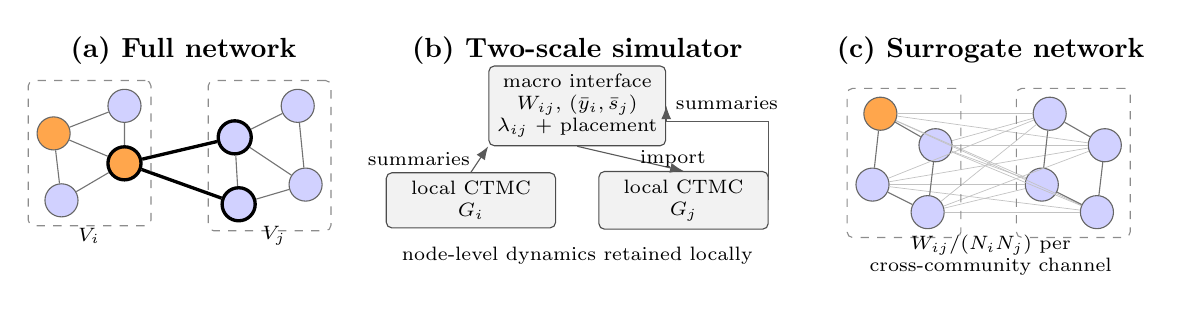
\begin{tikzpicture}[
  x=1cm,y=1cm,
  font=\scriptsize,
  >=Latex,
  person/.style={circle,draw=black!60,fill=blue!18,minimum size=4.2mm,inner sep=0pt},
  infected/.style={person,fill=orange!70},
  bridge/.style={person,very thick,draw=black},
  bridgeinf/.style={infected,very thick,draw=black},
  commbox/.style={draw=black!45,dashed,rounded corners=2pt,inner sep=3pt},
  macrobox/.style={draw=black!70,rounded corners=2pt,fill=black!5,align=center,inner sep=3pt},
  link/.style={draw=black!55},
  weak/.style={draw=black!24,line width=.25pt},
  flow/.style={-{Latex[length=1.7mm]},draw=black!65}
]
% (a) Full microscopic interface
\node[font=\bfseries] at (0,2.25) {(a) Full network};
\node[infected] (a1) at (-1.65,1.20) {};
\node[person]   (a2) at (-1.55,0.35) {};
\node[bridgeinf](a3) at (-0.75,0.82) {};
\node[person]   (a4) at (-0.75,1.55) {};
\node[bridge]   (b1) at (0.65,1.15) {};
\node[person]   (b2) at (1.45,1.55) {};
\node[person]   (b3) at (1.55,0.55) {};
\node[bridge]   (b4) at (0.70,0.30) {};
\draw[link] (a1)--(a2)--(a3)--(a1) (a1)--(a4)--(a3);
\draw[link] (b1)--(b2)--(b3)--(b4)--(b1) (b1)--(b3);
\draw[very thick] (a3)--(b1);
\draw[very thick] (a3)--(b4);
\node[commbox,fit=(a1)(a2)(a3)(a4)] {};
\node[commbox,fit=(b1)(b2)(b3)(b4)] {};
\node at (-1.2,-0.10) {$V_i$};
\node at (1.15,-0.10) {$V_j$};

% (b) Two-scale representation
\node[font=\bfseries] at (5.0,2.25) {(b) Two-scale simulator};
\node[macrobox] (macro) at (5.0,1.55) {macro interface\\$W_{ij}$, $(\ibar_i,\sbar_j)$\\$\lambda_{ij}$ + placement};
\node[macrobox,minimum width=2.15cm,minimum height=.70cm] (li) at (3.65,0.35) {local CTMC\\$G_i$};
\node[macrobox,minimum width=2.15cm,minimum height=.70cm] (lj) at (6.35,0.35) {local CTMC\\$G_j$};
\draw[flow] (li.north) -- node[left] {summaries} (macro.south west);
\draw[flow] (macro.south) -- node[right] {import} (lj.north);
\draw[flow] (lj.east) -- ++(0,1.0) -| node[pos=1.08,right] {summaries} (macro.east);
\node at (5.0,-0.35) {node-level dynamics retained locally};

% (c) Surrogate interface
\node[font=\bfseries] at (10.25,2.25) {(c) Surrogate network};
\node[infected] (c1) at (8.85,1.45) {};
\node[person]   (c2) at (8.75,0.55) {};
\node[person]   (c3) at (9.55,1.05) {};
\node[person]   (c4) at (9.45,0.20) {};
\node[person]   (d1) at (11.00,1.45) {};
\node[person]   (d2) at (10.90,0.55) {};
\node[person]   (d3) at (11.70,1.05) {};
\node[person]   (d4) at (11.60,0.20) {};
\foreach \u in {c1,c2,c3,c4}{\foreach \v in {d1,d2,d3,d4}{\draw[weak] (\u)--(\v);}}
\draw[link] (c1)--(c2)--(c4)--(c3)--(c1);
\draw[link] (d1)--(d2)--(d4)--(d3)--(d1);
\node[commbox,fit=(c1)(c2)(c3)(c4)] {};
\node[commbox,fit=(d1)(d2)(d3)(d4)] {};
\node[align=center] at (10.25,-0.35) {$W_{ij}/(N_iN_j)$ per\\cross-community channel};
\end{tikzpicture}
\caption{Схема міжспільнотного інтерфейсу. (a) У повній мережі інфекція переходить лише явними каналами, що примикають до вузлів-мостів. (b) У двомасштабному симуляторі кожна спільнота зберігає локальний рушій Gillespie/CTMC, а макроінтерфейс використовує зведення стану та агреговану вагу $W_{ij}$ для визначення інтенсивності імпорту й розміщення цільового вузла. (c) За рівномірного розміщення ідеальний двомасштабний процес еквівалентний сурогатній мережі з Твердження~\ref{prop:surrogate}, у якій кожна орієнтована міжспільнотна пара вузлів має слабку інтенсивність $\beta_{\mathrm{out}}W_{ij}/(N_iN_j)$. Помаранчеві вузли інфіковані, сині сприйнятливі.}
\label{fig:schematic}
\end{figure}

\subsection{Локальні рушії}
\label{sec:local}

Кожна спільнота моделюється окремим рушієм, який генерує траєкторії CTMC її власного графа $G_i$: зараження вздовж каналів у $E_{ii}$ та видалення інфікованих вузлів зі схильностями з~\eqref{eq:full_generator}, обмеженими на $V_i$. Рушії використовують інкрементну реалізацію Gillespie з \citet{kuryliak2025simulating}, у якій кожен вузол зберігає сумарну вагу своїх контактів з інфікованими сусідами, а оновлюються лише схильності, на які вплинула подія. Кожен рушій має власний незалежний потік псевдовипадкових чисел.

Рушій підтримує дві операції для макрорівня: просування годинника до заданого часу із застосуванням лише подій, що відбулися раніше, та \emph{імпорт} --- переведення заданого сприйнятливого вузла у стан $I$. Імпорт змінює локальний стан та інтенсивності, тому рушій відкидає заплановану подію й генерує нову з оновленого стану. Такий перезапуск статистично коректний для CTMC, оскільки відповідні часи очікування експоненційні. Еквівалентно, реалізація через випадкову заміну часу може зберегти невикористаний бюджет експоненційної інтенсивності після імпорту. За умови повної послідовності часів імпорту й цільових вузлів локальний рушій точно відтворює CTMC внутрішньоспільнотної мережі з цими імпортами як зовнішніми стрибками $S\to I$. Апроксимація виникає у способі генерування імпортів, а не в локальному моделюванні CTMC.

\subsection{Макрорівень}
\label{sec:macro}

Макрорівень розглядає спільноти як вузли зваженого графа з вагами $W_{ij}$. За поточними узагальненнями стану він призначає кожній упорядкованій парі $i\neq j$ інтенсивність
\begin{equation}
\label{eq:macro_rate}
\lambda_{ij}(t)=\beta_{\mathrm{out}}\,W_{ij}\,\ibar_i(t)\,\sbar_j(t),
\qquad
\Theta(t)=\sum_{i\neq j}\lambda_{ij}(t).
\end{equation}
Макроподія означає один імпорт інфекції з однієї спільноти до іншої. За умови макроподії в час $t$, коли $\Theta(t)>0$, пару $(i,j)$ вибирають з імовірністю $\lambda_{ij}(t)/\Theta(t)$, а цільовий вузол $v\in S_j(t)$ --- за правилом розміщення $\Pi_{ij}(\cdot\mid X(t))$. У всій статті використано рівномірне правило $\Pi_{ij}(v\mid X(t))=1/s_j(t)$. За наявності такої інформації можливі правила, зважені за степенем або з урахуванням межі. Реалізація також має мультиплікативний калібрувальний коефіцієнт для~\eqref{eq:macro_rate}; в усіх експериментах його встановлено рівним одиниці.

Рівняння~\eqref{eq:macro_rate} задає ефективну агреговану інтенсивність, а не, загалом, точну інтенсивність реалізованого мікроскопічного пучка. За фіксованих кількостей вузлів у станах вона дорівнює математичному сподіванню інтенсивності пучка, якщо кінцеві вузли міжспільнотних ребер рівномірно розміщені випадково й ми ще не враховуємо їхні конкретні ідентичності. Інтенсивності збігаються для рівномірного зв'язку «усі з усіма» (Наслідок~\ref{cor:exact}), а в інших випадках агрегована величина є наближенням (Розділ~\ref{sec:analysis}). Макрорівень не автономний: $\Theta$ змінюється після локальної події або імпорту, що змінює кількість вузлів у станах. Оскільки між такими подіями зведення стану кусково сталі, $\Theta$ також кусково стала.

\subsection{Час за інтегралом інтенсивності та синхронізація}
\label{sec:timing}

Нехай $t_0$ --- час попередньої макроподії, а $E\sim\Exp(1)$ --- незалежний поріг. В ідеальній конструкції наступна макроподія відбувається в момент
\begin{equation}
\label{eq:hazard_integral}
t^\ast=\inf\Bigl\{t>t_0:\int_{t_0}^{t}\Theta(s)\,ds\ge E\Bigr\},
\end{equation}
За фіксованих траєкторій мікрорівня $\Theta(t)$ є передбачуваною інтенсивністю, а конструкція~\eqref{eq:hazard_integral} відповідає поданню через випадкову заміну часу, або накопичену інтенсивність, \citep{ethier1986,anderson2007}. Безумовно процес макроподій має стохастичну передбачувану інтенсивність, а не детерміновану інтенсивність звичайного неоднорідного пуассонівського процесу. Для сталої $\Theta$ рівняння~\eqref{eq:hazard_integral} зводиться до часу очікування Gillespie $(t^\ast-t_0)=-\ln U/\Theta$, $U\sim\mathcal{U}(0,1)$. У поєднанні з точними локальними рушіями ця побудова визначає \emph{ідеальний} двомасштабний процес, характеристики переходів якого наведено в Розділі~\ref{sec:surrogate}.

Реалізований планувальник (Алгоритм~\ref{alg:scheduler}) трактує локальні рушії як «чорні скриньки», що відкривають свій стан лише після просування. Він ділить час на інтервали синхронізації довжини $\tau$. Позначимо через $A$ наближений накопичений макрорівневий hazard від попередньої макроподії. На кожному (під)інтервалі $[t,t_g)$, де $\Delta=t_g-t$, планувальник оцінює $\Theta$ пробою в середній точці: копії всіх рушіїв, разом зі станами їхніх генераторів випадкових чисел, просуваються до $t+\Delta/2$, де $\Delta=t_g-t$, після чого за копіями обчислюється $\Theta_{\mathrm{mid}}$. Якщо накопичена інтенсивність $A+\Theta_{\mathrm{mid}}\Delta$ залишається нижчою за $E$, фактичні рушії просуваються до $t_g$. Інакше момент перетину інтерполюється як
\begin{equation}
\label{eq:interpolation}
t^\ast=t+\frac{E-A}{\Theta_{\mathrm{mid}}},
\end{equation}
рушії просуваються до $t^\ast$, а пару та цільовий вузол вибирають за їхніми станами в момент $t^\ast$. Потім поріг поновлюється, й у такий самий спосіб обробляється решта інтервалу.

\begin{algorithm}[tbp]
\caption{Сітково синхронізоване двомасштабне моделювання однієї реалізації.}
\label{alg:scheduler}
\small
\begin{tabbing}
\hspace*{1.6em}\=\hspace*{1.4em}\=\hspace*{1.4em}\=\hspace*{1.4em}\=\kill
\textbf{Вхід:} локальні графи $G_i$, ваги $W_{ij}$, інтенсивності, крок $\tau$, горизонт $T_{\mathrm{end}}$, початковий стан.\\[2pt]
1:\> $t\gets 0$;\ \ $A\gets 0$;\ \ згенерувати $E\sim\Exp(1)$\\
2:\> \textbf{while} $t<T_{\mathrm{end}}$ і інфекція ще може поширюватися \textbf{do}\\
3:\>\> $t_g\gets\min(t+\tau,\,T_{\mathrm{end}})$\\
4:\>\> \textbf{while} $t<t_g$ \textbf{do}\\
5:\>\>\> $\Delta\gets t_g-t$; скопіювати кожен рушій разом зі станом генератора випадкових чисел; просунути копії до $t+\Delta/2$\\
6:\>\>\> $\Theta_{\mathrm{mid}}\gets\sum_{i\neq j}\lambda_{ij}$, обчислена за копіями, рівняння~\eqref{eq:macro_rate}\\
7:\>\>\> \textbf{if} $A+\Theta_{\mathrm{mid}}\Delta<E$ \textbf{then} \hspace{1em}{\color{black!60}// до $t_g$ макроподій немає}\\
8:\>\>\>\> просунути всі рушії до $t_g$;\ \ $A\gets A+\Theta_{\mathrm{mid}}\Delta$;\ \ $t\gets t_g$\\
9:\>\>\> \textbf{else}\\
10:\>\>\>\> $t^\ast\gets t+(E-A)/\Theta_{\mathrm{mid}}$;\ \ просунути всі рушії до $t^\ast$\\
11:\>\>\>\> вибрати $(i,j)$ з імовірністю $\lambda_{ij}(t^\ast)/\Theta(t^\ast)$ за станами рушіїв\\
12:\>\>\>\> рівномірно вибрати $v$ з $S_j(t^\ast)$; імпортувати $v$ до рушія $j$ (його заплановану подію відкинути)\\
13:\>\>\>\> $t\gets t^\ast$;\ \ $A\gets 0$;\ \ згенерувати нове $E\sim\Exp(1)$
\end{tabbing}
\end{algorithm}

Для інтерпретації результатів важливі дві властивості планувальника. По-перше, оскільки проби копіюють стани генераторів випадкових чисел, проба відтворює траєкторію, якою відповідний рушій фактично просуватиметься до середньої точки, якщо не відбудеться імпорт. Тому проба в середній точці є квадратурою реалізованої кусково сталої інтенсивності. Вона точна на підінтервалах без локальних подій у жодній спільноті; похибка квадратури та випереджувальний перегляд не більш як на $\tau/2$ зникають при $\tau\to0$. По-друге, якщо локальні рушії повідомляють часи наступних подій, припущення «чорної скриньки» не потрібне. Оскільки $\Theta$ кусково стала між локальними подіями, інтеграл~\eqref{eq:hazard_integral} тоді можна точно обчислювати подієво керованим планувальником, який об'єднує часи наступних подій усіх рушіїв. Це усуває чисельну похибку синхронізації. В експериментах оцінюємо сітковий варіант із кроком $\tau=1$.

\subsection{Обчислювальна структура та передбачене застосування}
\label{sec:cost}

\Full{} зберігає кожен канал, зокрема всі міжспільнотні канали, а його вартість на одну подію зростає зі степенем вузла \citep{kuryliak2025simulating}. \TS{} зберігає внутрішньоспільнотні графи та матрицю ваг розміру $M\times M$. Саме цю економію підкреслено в матеріалах семінару \citep{kuryliak2025towards}: коли міжспільнотні контакти численні, наприклад коли потік мобільності відповідає багатьом індивідуальним контактам, інтерфейс зводиться до $O(M^2)$ чисел. Локальні рушії також можна змінювати незалежно, що спрощує подання втручань, специфічних для окремих спільнот. Водночас сітково синхронізований планувальник додає витрати, пропорційні $(T_{\mathrm{end}}/\tau)\sum_iN_i$, на копіювання станів рушіїв, незалежно від кількості подій. Отже, метод призначений для умов, у яких міжспільнотні контакти невідомі або надто численні для явного подання, а не для малих мереж із доступною повною структурою контактів. Виміряний час виконання наведено в Розділі~\ref{sec:disc_cost}.

%======================================================================

\clearpage
\section{Що агрегований інтерфейс зберігає, а що втрачає}
\label{sec:analysis}

\subsection{Представлення за допомогою сурогатної мережі}
\label{sec:surrogate}

За точного обчислення часу~\eqref{eq:hazard_integral} ідеальний двомасштабний процес є CTMC на $\{S,I,R\}^V$. Інтенсивність його переходу $x\to x^{v:I}$ унаслідок імпорту дорівнює $\sum_{i\neq j}\lambda_{ij}(x)\Pi_{ij}(v\mid x)$ для $v\in S_j(x)$; усі локальні переходи мають інтенсивності з~\eqref{eq:full_generator}, обмежені на $E_{ii}$. Наступне твердження ототожнює цей процес із процесом на повній мережі зі зміненим графом.

\begin{proposition}[Сурогатна мережа]
\label{prop:surrogate}
Нехай $\tilde G$ --- мережа з тими самими внутрішньоспільнотними каналами та інтенсивностями, що й $G$, у якій кожен міжспільнотний пучок $E_{ij}$ замінено повною множиною каналів $V_i\times V_j$, кожен з інтенсивністю $\tilde\beta_{uv}=\beta_{\mathrm{out}}W_{ij}/(N_iN_j)$. За рівномірного розміщення ідеальний двомасштабний процес має генератор $\mathcal{L}_{\tilde G}$; тобто він має закон процесу на повній мережі $\tilde G$, запущеного з тієї самої конфігурації.
\end{proposition}

\begin{proof}
Видалення та внутрішньоспільнотні зараження мають однакові інтенсивності в обох процесах. Розглянемо сприйнятливий вузол $v\in V_j$ у конфігурації $x$. За рівномірного розміщення двомасштабна інтенсивність, з якою $v$ заражається внаслідок імпорту, дорівнює
\[
\sum_{i\neq j}\lambda_{ij}(x)\,\frac{1}{s_j(x)}
=\sum_{i\neq j}\beta_{\mathrm{out}}W_{ij}\frac{y_i(x)}{N_i}\frac{s_j(x)}{N_j}\frac{1}{s_j(x)}
=\sum_{i\neq j}\sum_{u\in V_i}\frac{\beta_{\mathrm{out}}W_{ij}}{N_iN_j}\ind\{x_u=I\},
\]
що є сумарною інтенсивністю міжспільнотних каналів $\tilde G$, спрямованих у $v$. Коли $s_j(x)=0$, обидві інтенсивності дорівнюють нулю. Отже, всі інтенсивності переходів збігаються, а генератори є однаковими. \qed
\end{proof}

\begin{corollary}
\label{cor:exact}
Якщо кожен міжспільнотний пучок у $G$ уже є повним, $E_{ij}=V_i\times V_j$, зі спільною інтенсивністю для кожної пари спільнот, тоді $\tilde G=G$, а ідеальний двомасштабний процес є точним.
\end{corollary}

Сурогатна мережа зберігає сумарну вагу кожного пучка, $\sum_{(u,v)\in V_i\times V_j}\tilde\beta_{uv}=\beta_{\mathrm{out}}W_{ij}$, але рівномірно розподіляє її між усіма парами (рисунок~\ref{fig:schematic}c). Тому похибка апроксимації ідеального методу є різницею між епідеміями на $G$ та $\tilde G$, які відрізняються лише своїми інтерфейсами. Реалізований метод додає чисельну похибку синхронізації. Твердження~\ref{prop:surrogate} також дає практичний спосіб верифікації: для малих мереж похибку синхронізації можна виокремити, порівнюючи двомасштабний симулятор із точною симуляцією на $\tilde G$.

\subsection{Джерела розбіжностей}
\label{sec:sources}

Порівняння $G$ із $\tilde G$ виявляє чотири механізми, через які двомасштабний симулятор може відхилятися від процесу на повній мережі.

\paragraph{Інформація про стан межі (з боку джерела).}
У $G$ інтенсивність передавання з $V_i$ до $V_j$ дорівнює
\begin{equation}
\label{eq:exact_rate}
a^\star_{ij}(x)=\beta_{\mathrm{out}}\sum_{(u,v)\in E_{ij}}w_{uv}\,\ind\{x_u=I,\,x_v=S\},
\end{equation}
і залежить від того, чи заражені конкретні мостові вузли. У $\tilde G$ свій внесок робить кожен заражений вузол $V_i$. Тому експорти можуть відбуватися до зараження будь-якого мостового вузла. Такий \emph{обхід мостів} неможливий у $G$ і дає безпосередній діагностичний показник (розділ~\ref{sec:single_export}).

\paragraph{Розміщення (з боку приймача).}
У $G$ передавання заражає цільову кінцеву вершину каналу, що спрацював; у $\tilde G$ ціль рівномірно вибирається серед сприйнятливих вузлів. Місце імпорту визначає його відстань до наступного інтерфейсу, а отже, і час подальших переходів.

\paragraph{Вичерпання інтерфейсу (з боку приймача).}
За SI-динаміки канал $G$ передає зараження не більш ніж один раз: після цього його ціль заражена. Тому пучок із $|E_{ij}|$ каналів переносить не більш ніж $|E_{ij}|$ заражень, а інтерфейс з одним ребром --- рівно одне. У $\tilde G$ імпорти з $V_i$ у $V_j$ тривають з інтенсивністю $\lambda_{ij}=\beta_{\mathrm{out}}W_{ij}\ibar_i\sbar_j$, доки $V_j$ не буде вичерпано; їхня очікувана кількість за період $[t_1,t_2]$ дорівнює $\mathbb{E}\int_{t_1}^{t_2}\lambda_{ij}(s)\,ds$. Отже, коли приймальна спільнота тривалий час залишається переважно сприйнятливою, двомасштабний симулятор продовжує засівати її додатковими зараженнями, яких повна мережа передати не може.

\paragraph{Синхронізація.}
Квадратурна формула середньої точки та інтерполяція з розділу~\ref{sec:timing} апроксимують~\eqref{eq:hazard_integral}.

\begin{remark}[Розміщення за рандомізованих інтерфейсів]
\label{rem:placement}
Припустімо, що кінцеві вершини кожного пучка вибираються рівномірно й незалежно від внутрішніх графів та кінцевих вершин інших пучків, як у наведених нижче експериментах. Тоді ціль першого передавання до повністю сприйнятливої спільноти має рівномірний розподіл і в $G$, оскільки вона є кінцевою вершиною рівномірно розміщеного каналу, і в $\tilde G$. Тому розміщення може впливати на часи прибуття лише через передавання після першого. У таких схемах відмінності між першим і подальшими переходами виокремлюють ефекти з боку приймача (розділ~\ref{sec:res_descriptor}).
\end{remark}

\subsection{Одиничний експорт: стохастичне впорядкування та обхід мостів}
\label{sec:single_export}

Розглянемо спільноту-джерело $V_0$ розміру $n$ із довільним внутрішнім графом, SI-динамікою та єдиним сприйнятливим листковим вузлом $\ell$, сполученим із множиною $B\subset V_0$ з $k$ мостових вузлів каналами з інтенсивністю $\beta_{\mathrm{out}}$. Тоді $W_{0\ell}=k$, а до експорту $\sbar_\ell=1$, тому $\lambda_{0\ell}=\beta_{\mathrm{out}}k\,\ibar_0$. Нехай $\tau_u$ --- час зараження вузла $u$, $A_u(t)=(t-\tau_u)^+$ --- тривалість його перебування в зараженому стані, а $T_B=\min_{u\in B}\tau_u$.

\begin{proposition}[Агреговані годинники експорту спрацьовують раніше]
\label{prop:ordering}
Нехай $B$ має рівномірний розподіл на множині всіх $k$-елементних підмножин $V_0$ незалежно від внутрішнього графа, початкової конфігурації та випадковості подій. Нехай $T^{\Full}$ і $T^{\TS}$ --- часи першого зараження $\ell$ відповідно в повній мережі та в ідеальному двомасштабному процесі. Тоді
\[
\mathbb{P}(T^{\Full}>t)\;\ge\;\mathbb{P}(T^{\TS}>t)\qquad\text{for all }t\ge0,
\]
отже, $T^{\TS}$ є стохастично меншим за $T^{\Full}$ \citep{shaked2007}. Зокрема, середнє та кожен квантиль часу експорту ідеального двомасштабного процесу не перевищують відповідних величин часу експорту в повній мережі.
\end{proposition}

\begin{proof}
До зараження $\ell$ не впливає на $V_0$: він нічого не передає, а інтенсивності вузлів джерела залежать лише від їхніх заражених сусідів. Тому обидва часи експорту можна побудувати на одному ймовірнісному просторі з автономної SI-траєкторії $X_0$ спільноти-джерела, продовженої після експорту, та незалежного порога $E\sim\Exp(1)$:
\[
T^{\Full}=\inf\Bigl\{t:\beta_{\mathrm{out}}\sum_{u\in B}A_u(t)\ge E\Bigr\},\qquad
T^{\TS}=\inf\Bigl\{t:\beta_{\mathrm{out}}\frac{k}{n}\sum_{u\in V_0}A_u(t)\ge E\Bigr\},
\]
де другий підінтегральний вираз випливає з $\int_0^t\ibar_0(s)\,ds=n^{-1}\sum_uA_u(t)$. Умовні щодо $X_0$ ймовірності виживання дорівнюють $\exp(-\beta_{\mathrm{out}}\sum_{u\in B}A_u(t))$ та $\exp(-\beta_{\mathrm{out}}(k/n)\sum_uA_u(t))$. Оскільки $B$ є рівномірною та незалежною від $X_0$, маємо $\mathbb{E}[\sum_{u\in B}A_u(t)\mid X_0]=(k/n)\sum_uA_u(t)$, а нерівність Єнсена для опуклої функції $z\mapsto e^{-\beta_{\mathrm{out}}z}$ дає $\mathbb{P}(T^{\Full}>t\mid X_0)\ge\mathbb{P}(T^{\TS}>t\mid X_0)$. Взяття математичного сподівання завершує доведення. \qed
\end{proof}

Нерівність є строгою, якщо з додатною ймовірністю тривалості перебування вузлів у зараженому стані в момент $t$ відрізняються та $0<k<n$. Вона також виконується, коли $B$ рівномірно розподілена серед вузлів, відмінних від початково зараженого, оскільки вилучення вузла, зараженого найдавніше, може лише зменшити умовне середнє мостової небезпеки. Величина розриву визначається умовною дисперсією мостової небезпеки, для якої вибірка без повернення дає
\begin{equation}
\label{eq:hazard_variance}
\operatorname{Var}\Bigl(\beta_{\mathrm{out}}\sum_{u\in B}A_u(t)\Bigm| X_0\Bigr)=\beta_{\mathrm{out}}^2\,k\,\frac{n-k}{n-1}\,\operatorname{Var}_u\bigl(A_u(t)\bigr),
\end{equation}
де $\operatorname{Var}_u$ --- генеральна дисперсія за вузлами джерела. Після повного зараження джерела $\operatorname{Var}_u(A_u(t))=\operatorname{Var}_u(\tau_u)$. Отже, агрегований годинник є близьким до точного, коли часи зараження вузлів зосереджені порівняно з $1/\beta_{\mathrm{out}}$, як у кліці, що швидко насичується, і спрацьовує раніше, коли зараження поширюється джерелом повільно й нерівномірно.

Та сама побудова дає ймовірність обходу мостів. У $G$ експорт не може передувати $T_B$. В ідеальному двомасштабному процесі
\begin{equation}
\label{eq:bypass}
\mathbb{P}\bigl(T^{\TS}<T_B\bigr)=\mathbb{E}\Bigl[1-\exp\Bigl(-\beta_{\mathrm{out}}\frac{k}{n}\int_0^{T_B}y_0(s)\,ds\Bigr)\Bigr],
\end{equation}
що є ймовірністю того, що агрегована небезпека, накопичена до активації справжнього інтерфейсу, спричинить експорт. Вона зростає, коли зараження досягає мостів пізно та після багатьох інших вузлів, як це відбувається в розріджених спільнотах із довгими шляхами. Додаток~\ref{app:clique} наводить $\mathbb{E}[T_B]$ для джерела-кліки.

\subsection{Характеристика співвідношення часових масштабів}
\label{sec:descriptor}

Механізми як з боку джерела, так і з боку приймача діють лише доти, доки зараження ще поширюється всередині спільноти. Згідно з~\eqref{eq:hazard_variance}, розрив з боку джерела визначається добутком $\beta_{\mathrm{out}}$ і розсіювання часів зараження. Очікувана кількість надлишкових імпортів до спільноти під час внутрішнього поширення має порядок $\beta_{\mathrm{out}}W_{ij}$, помножений на тривалість цього поширення. Нехай $\sigma_T$ позначає стандартне відхилення часів зараження вузлів усередині спільноти, яке вимірює цю тривалість. Як характеристику очікуваної точності ми використовуємо безрозмірне співвідношення
\begin{equation}
\label{eq:rho}
\rho=\beta_{\mathrm{out}}\,\sigma_T,
\end{equation}
тобто внутрішній розкид часу в одиницях середнього часу переходу через одне ребро $1/\beta_{\mathrm{out}}$. Ці два механізми по-різному масштабуються із шириною інтерфейсу ($\sqrt{k}$ у~\eqref{eq:hazard_variance} та $k$ для надлишкових імпортів, що частково компенсується тим, що сама повна мережа допускає до $k$ переходів). Тому ми не включаємо $k$ до $\rho$ та перевіряємо цю характеристику емпірично, а не виводимо закон похибки.

%======================================================================
\clearpage
\section{Дизайн експерименту}
\label{sec:design}

\subsection{Тестові задачі}

У таблиці~\ref{tab:design} підсумовано чотири серії експериментів. Усі вони використовують SI-динаміку, одиничні ваги контактів, однакові внутрішні й зовнішні інтенсивності на ребро ($\beta_{\mathrm{in}}=\beta_{\mathrm{out}}=\beta$) та планувальник з алгоритму~\ref{alg:scheduler} з $\tau=1$. У тестовій задачі \emph{кліка--листок} листок приєднано до $k=2$ мостових вузлів кліки зі 100 вузлів. У \emph{переборі джерело--листок} кліку замінено зв'язними випадковими графами з $n=1000$ вузлів із заданою середньою довжиною найкоротшого шляху (ASPL). У серії \emph{ланцюг} $L=10$ спільнот з'єднано в лінію за допомогою $k$ ребер між послідовними спільнотами; зараження починається у спільноті 0. Зв'язні випадкові графи генеруються додаванням рівномірно випадкових ребер до рівномірно випадкового дерева з міченими вершинами; кількість доданих ребер калібрується так, щоб ASPL лежала в межах 0.1 від цільового значення; ASPL 1 відповідає повному графу. Тому середній степінь зменшується зі зростанням цільової ASPL. За цільової ASPL 6 він змінюється від 2.08 для $n=50$ до 3.4 для $n=1000$. Кінцеві вершини інтерфейсів вибираються рівномірно й незалежно для кожного інтерфейсу та повтору.\footnote{У переборі джерело--листок множини мостів вибираються з усіх вузлів, крім одного вузла з фіксованою міткою. Оскільки випадкові графи та рівномірно вибране початкове зараження є інваріантними за законом відносно перемічування міток, це еквівалентно рівномірному розміщенню, тож припущення твердження~\ref{prop:ordering} виконується.} Початковий заражений вузол є псевдовипадковим і спільним для обох симуляторів; він може бути мостовим вузлом. У тестовій задачі кліка--листок початковим є фіксований вузол кліки.

\clearpage
\begin{table}[H]
\centering
\caption{Серії експериментів. Кожна комірка перебору використовує 40 реалізацій мережі (блоків) із 10 повторами інтерфейсу та подій у кожній. ASPL: цільова внутрішня середня довжина найкоротшого шляху (1 позначає повний граф).}
\label{tab:design}
\small
\begin{tabular}{>{\raggedright\arraybackslash}p{0.17\linewidth}>{\raggedright\arraybackslash}p{0.36\linewidth}>{\raggedright\arraybackslash}p{0.06\linewidth}>{\raggedright\arraybackslash}p{0.08\linewidth}>{\raggedright\arraybackslash}p{0.2\linewidth}}
\toprule
Серія & Структура & $k$ & $\beta$ & Запусків на комірку та модель\\
\midrule
Кліка--листок & кліка-джерело $n=100$ $+$ один листок & 2 & 0.005 & 10\,000\\
Перебір джерело--листок & джерело $n=1000$, ASPL 1--6 із кроком 0.25, $+$ один листок & 1, 5 & 0.003 & 400 (40 $\times$ 10)\\
Ланцюг клік & $L=10$ клік із $n=1000$ & 1 & 0.003 & 400 (40 $\times$ 10)\\
Перебір розміру ланцюга & $L=10$, $n\in\{50,100,250,1000\}$, ASPL 1--6 із кроком 1 & 1, 5 & 0.003 & 400 (40 $\times$ 10)\\
\bottomrule
\end{tabular}
\end{table}

Запуски \Full{} та \TS{} є зіставленими: вони мають спільні граф, інтерфейс і початковий вузол, але використовують незалежні потоки подій. Усі експорти та прибуття, що входять до метрик, було спостережено, тому поправка на цензурування не потрібна. Горизонт становив 1000 для тестової задачі кліка--листок та 30\,000 для решти. Два запуски \Full{} було продовжено до 40\,000, щоб спостерегти їхні термінальні прибуття (додаток~\ref{app:repro}). Ланцюг клік є коміркою ASPL-1, $n=1000$, $k=1$ перебору розміру, поданою окремо, оскільки це найсприятливіший випадок.

\subsection{Спостережувані величини та метрики}

Для тестових задач із листком ми реєструємо час експорту $T_{\mathrm{export}}$ (перше зараження листка) та час активації мосту $T_B$. Для ланцюгів $T_c$ --- час першого зараження спільноти $c$, відрахований від початкового зараження; термінальне прибуття --- це $T_9$. Ми подаємо три підсумкові показники:
\begin{itemize}
\item відносний зсув медіани $b_c=100\,[\mathrm{med}(T^{\TS}_c)-\mathrm{med}(T^{\Full}_c)]/\mathrm{med}(T^{\Full}_c)$, де від'ємні значення означають раніше прибуття в \TS{};
\item відносну відстань Вассерштайна-1 $\eW=100\,W_1/\overline{T}^{\Full}$, де $W_1=R^{-1}\sum_r|T^{\TS}_{(r)}-T^{\Full}_{(r)}|$ обчислюється за порядковими статистиками $R$ часів кожної моделі;
\item частку обходу мостів, тобто відсоток переходів у \TS{}, що відбуваються до зараження будь-якого мостового вузла спільноти-джерела.
\end{itemize}
Для ланцюгів \emph{локальний} зсув переходу $c$ порівнює середні значення $T_c-T_{c-1}$ між моделями. Ми зіставляємо перший перехід з об'єднаними переходами 2--9, використовуючи $T_9-T_1$.

\subsection{Статистичні процедури}

Довірчі інтервали є 95\% процентильними інтервалами з бутстрепу, який повторно вибирає цілі мережеві блоки, зберігаючи разом їхні десять повторів; для підсумкових показників ланцюга використовуються 2000 бутстреп-вибірок. Оскільки $\eW$ є додатною навіть тоді, коли дві вибірки походять з одного закону розподілу, ми калібруємо її за допомогою перестановочного тесту всередині пар: мітки двох запусків у кожній зіставленій парі міняються місцями з імовірністю $1/2$, після чого $\eW$ повторно обчислюється 2000 разів. За нульової гіпотези про обмінність зіставлених запусків це дає вибірковий нижній поріг, який ми підсумовуємо його 95-м процентилем, а також $p$-значення для спостережуваної $\eW$. Додаток~\ref{app:floor} наводить аналітичне наближення цього порога, застосовне, коли дані окремих запусків недоступні.

Початкові значення генератора подій для повтору залежать від цільової ASPL, мережевого блоку та індексу повтору, але не від $n$ або $k$; отже, початкові значення є спільними для різних розмірів спільноти та ширин інтерфейсу (спільні випадкові числа). Це зменшує дисперсію порівнянь між такими комірками, але також корелює їхні похибки вибірки. Тому ми не вважаємо узгодженість між комірками незалежним повторенням.

\subsection{Верифікація еталонної моделі}
\enlargethispage{2\baselineskip}

Для джерела-кліки з рівномірно розміщеними мостами очікуваний час активації мосту відомий у замкненій формі (додаток~\ref{app:clique}). Для чотирьох розмірів ланцюга клік і обох ширин інтерфейсу середнє $T_B$ у \Full{} узгоджувалося з формулою в межах 2.3 стандартної похибки. Для $k=1$ середній час очікування після активації мосту (326.5--354.0) узгоджувався з точним значенням $1/\beta=333.3$ у межах похибки вибірки (таблиця~\ref{tab:verification}).

%======================================================================

\clearpage
\section{Результати}
\label{sec:results}

\subsection{Одиничний експорт із кліки}
\label{sec:res_clique}

\emph{Часи експорту з джерела, яке швидко насичується, добре узгоджуються, але агрегований інтерфейс допускає неможливі порядки передачі.} У тесті «кліка--листок» (рисунок~\ref{fig:clique_leaf}) середні часи експорту становили 110.18 (\Full{}) і 112.62 (\TS{}); парна різниця $+2.43$ мала бутстреп-інтервал $[-0.35,5.27]$. Емпіричні функції розподілу майже збігаються ($W_1=3.25$, тобто $\eW=2.95\%$; відстань Колмогорова--Смирнова 0.0142, асимптотичне $p\approx0.27$). Із середнього часу експорту близько 110 лише $\mathbb{E}[T_B]=8.36$ у середньому потрібно, щоб заразити перший вузол-мост~\eqref{eq:clique_TB}; решта припадає на очікування передачі через інтерфейс з інтенсивністю не більшою за $k\beta=0.01$. Отже, період, протягом якого стани межі й усієї спільноти відрізняються, короткий, а агрегований годинник близький до точного, як випливає з твердження~\ref{prop:ordering} та~\eqref{eq:hazard_variance}.

Водночас діагностика порядку розрізняє моделі: у 98 із 10\,000 запусків \TS{} (0.98\%) листок було заражено раніше за обидва вузли-мости, чого ніколи не трапляється у \Full{} (рисунок~\ref{fig:clique_leaf}b,c). На середній панелі показано $T_{\mathrm{export}}-T_B$: фізичний час очікування у \Full{}, але знаковий діагностичний показник порядку у \TS{}.

\clearpage
\begin{figure}[H]
\centering
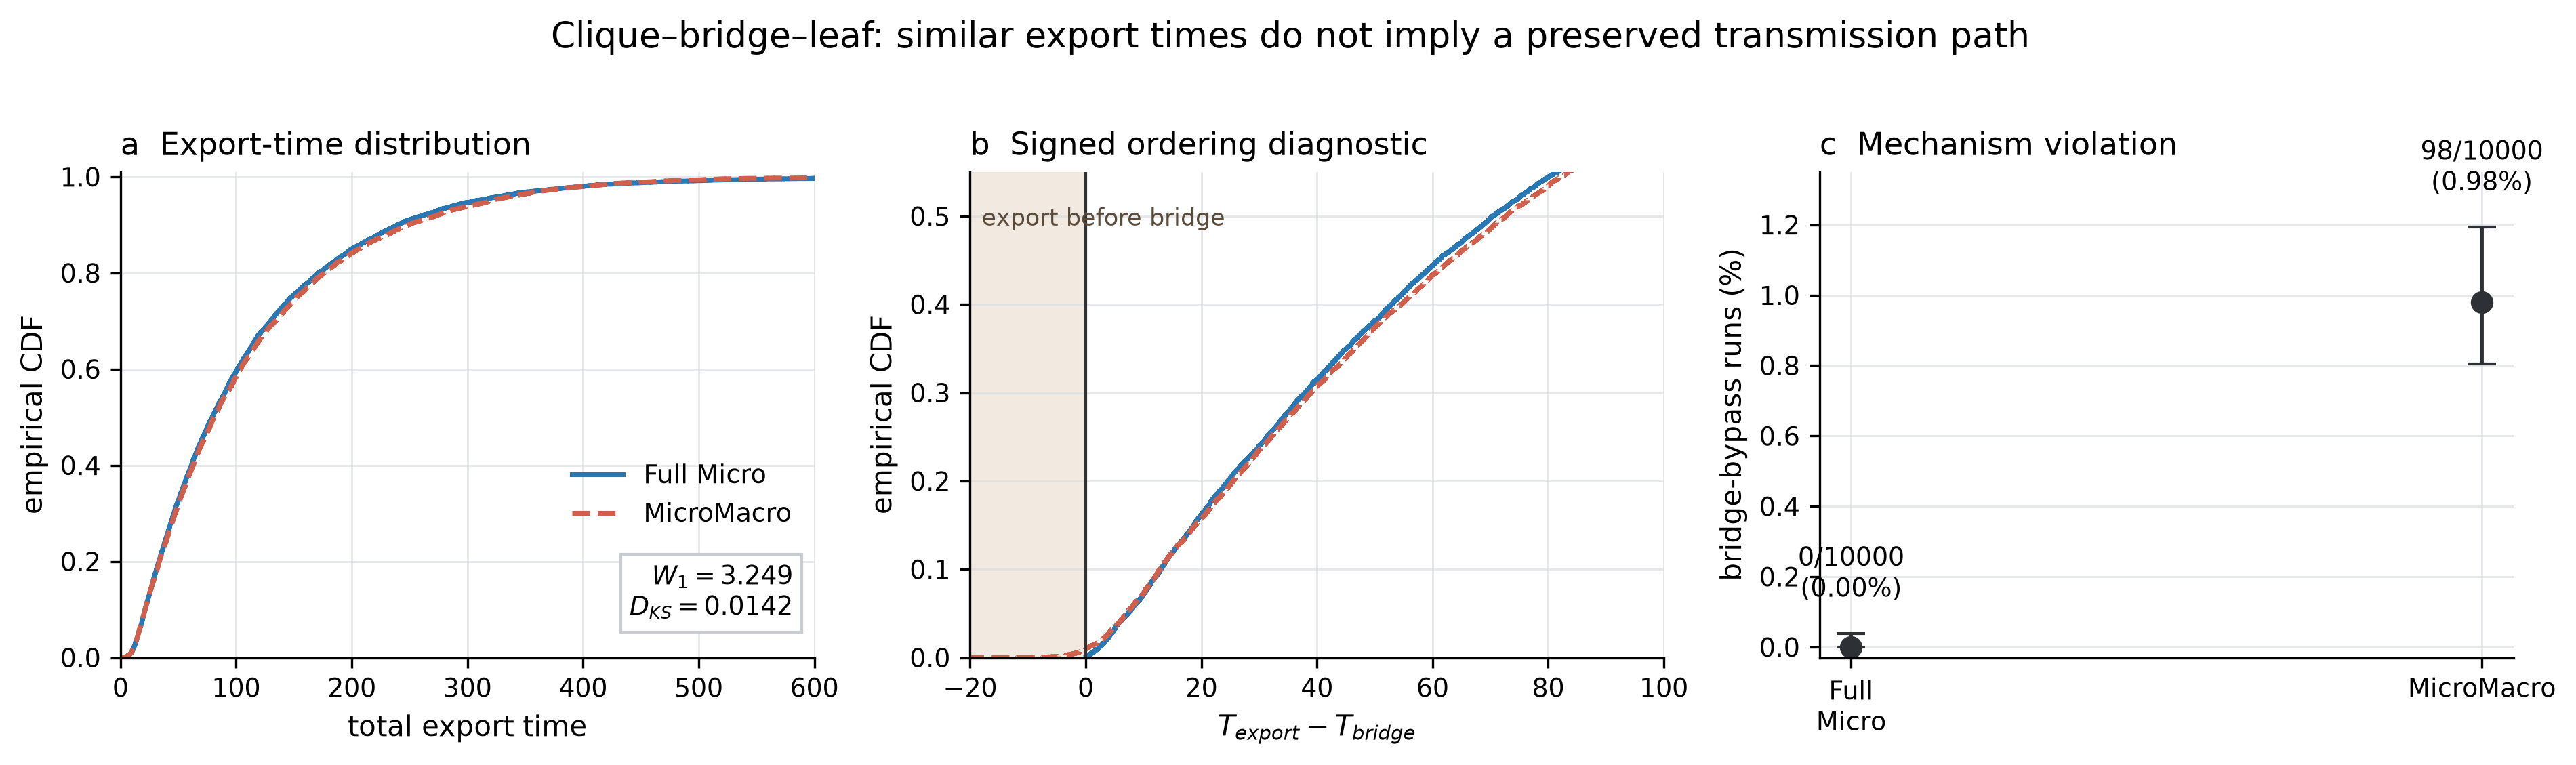
\includegraphics[width=\linewidth]{Images/clique_leaf/clique_leaf_endpoint_and_mechanism.png}
\caption{Тест «кліка--листок» ($n=100$, $k=2$, $\beta=0.005$, 10\,000 запусків для кожної моделі). (a) Емпіричні функції розподілу часу експорту. (b) Емпіричні функції розподілу $T_{\mathrm{export}}-T_B$; від'ємні значення (заштрихована область) відповідають експорту до зараження будь-якого вузла-моста. (c) Частка таких запусків з обходом мостів із 95\% інтервалами. ``Full Micro'' позначає \Full{}, а ``MicroMacro'' --- \TS{}.}
\label{fig:clique_leaf}
\end{figure}

\subsection{Одиничний експорт зі зв'язних випадкових джерел}
\label{sec:res_source}

\emph{Зі збільшенням довжини внутрішніх шляхів обхід мостів стає поширеним, а агрегований експорт відбувається раніше, як передбачає твердження~\ref{prop:ordering}.} На рисунку~\ref{fig:source_sweep} показано серію експериментів «джерело--листок». Середні часи активації мостів у двох моделях були подібними: різниця не перевищувала 7\% для кожного ASPL (наприклад, 1165 і 1136 за ASPL 6, $k=1$), як і очікувалося через однакову локальну динаміку до експорту. У \Full{} за $k=1$ очікування після активації моста залишалося в межах 322--359 за кожного ASPL, що узгоджується з $\mathrm{Exp}(\beta)$ із середнім 333. У \TS{} знаковий інтервал $T_{\mathrm{export}}-T_B$ ($k=1$) зменшився приблизно з 340 у щільних джерелах до 207--295 за ASPL $\ge5$, оскільки агрегована інтенсивність накопичувалася ще до того, як справжній міст ставав інфекційним.

\clearpage
\begin{figure}[H]
\centering
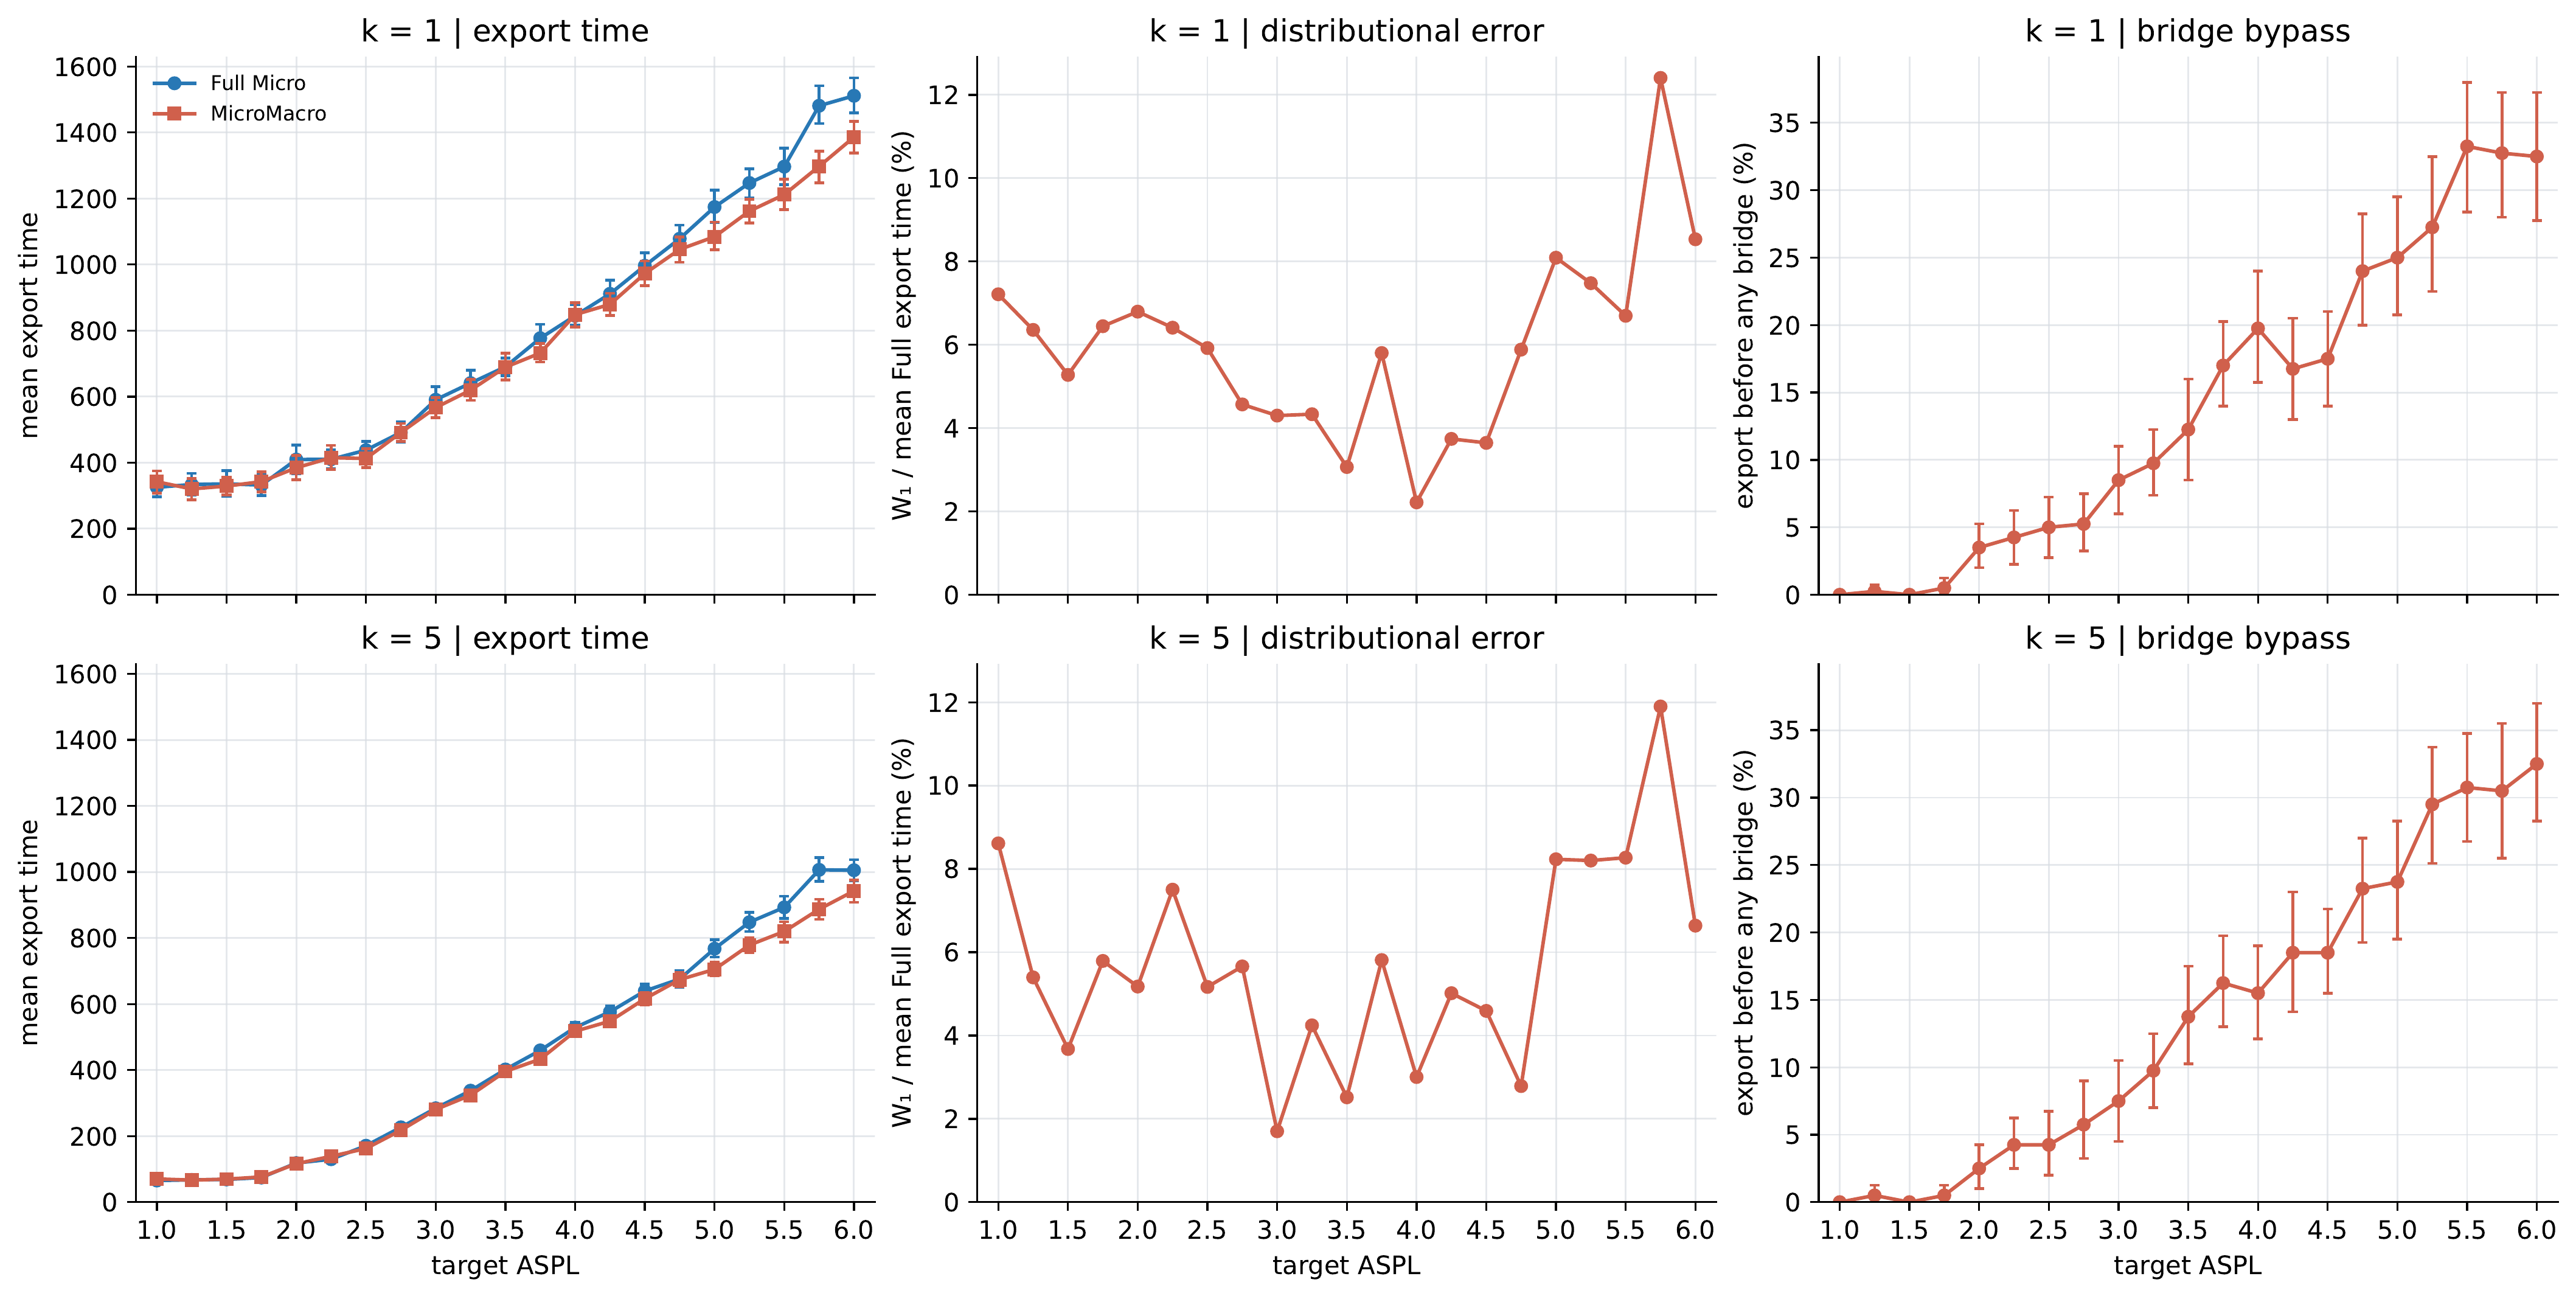
\includegraphics[width=\linewidth]{Images/fig_aspl_export_fidelity.png}
\caption{Серія експериментів «джерело--листок»: $n=1000$, $\beta=0.003$, $k=1$ (угорі) та $k=5$ (унизу), 400 парних запусків для кожної точки. Ліворуч: середній час експорту. У центрі: відносна відстань Васерштайна $\eW$ між розподілами часу експорту. Праворуч: частка експортів \TS{}, що передували зараженню першого моста; у \Full{} таких випадків не було. Відрізки похибок --- 95\% інтервали блокового бутстрепу. ``Full Micro'' позначає \Full{}, а ``Production MicroMacro'' --- \TS{}.}
\label{fig:source_sweep}
\end{figure}

Частка обходів зросла від не більш як 0.5\% за ASPL $\le1.75$ до 19.75\% (95\% інтервал 15.8--24.0\%) за ASPL 4 і $k=1$, а за ASPL 6 --- до 32.5\% для обох ширин інтерфейсу. Зсув середнього часу експорту був статистично відмінним від нуля, з інтервалами, що не містили нуль, для обох ширин за кожного ASPL $\ge5$. Його значення були в межах від $-6.2\%$ до $-12.4\%$; за ASPL 6 вони становили $-8.3\%$ ($[-13.1,-3.5]$) для $k=1$ і $-6.2\%$ ($[-10.3,-2.3]$) для $k=5$. Нижче ASPL 5 статистично відмінний від нуля зсув виявлено лише для $k=5$ за ASPL 3.75, 4.25 і 4.5 (від $-3.7\%$ до $-5.8\%$). У жодній точці серії не виявлено додатного зсуву, що узгоджується з напрямом, передбаченим твердженням~\ref{prop:ordering}.

Нерегулярну центральну панель слід тлумачити обережно. Для майже експоненційних часів експорту та $R=400$ запусків для кожної моделі очікуване $\eW$ двох вибірок з одного розподілу становить приблизно $\sqrt{\pi/R}\approx9\%$ (додаток~\ref{app:floor}). Отже, значення 3.7--8.6\%, спостережені за ASPL $\le1.75$, узгоджуються із суто вибірковою мінливістю. Тому відстані для одиничного експорту слід розглядати разом зі зсувом середнього та його інтервалом. Натомість обхід у \Full{} за побудовою дорівнює нулю, тому кожен спостережений обхід є справжньою розбіжністю. За ASPL 4 він стосується однієї п'ятої експортів, хоча розподіли часу експорту залишаються близькими.

\subsection{Повторні переходи через ланцюг клік}
\label{sec:res_cliques}

\emph{Коли внутрішнє поширення швидке, близьке узгодження зберігається після дев'яти послідовних агрегованих переходів.} У ланцюзі з десяти клік по 1000 вузлів із $k=1$ медіанний час прибуття до останньої спільноти становив 2785 у \Full{} і 2877 у \TS{}, а $\eW=3.34\%$ (рисунок~\ref{fig:chain_cliques}). Пермутаційний поріг для цієї комірки становив 5.1\% ($p=0.32$), тому два термінальні розподіли статистично нерозрізнювані. Функції розподілу перетинаються, отже різниця не є сталим запізненням. Кліка з 1000 вузлів у середньому насичується за $2H_{999}/(\beta n)\approx5$ одиниць часу, тоді як середній час переходу через ребро дорівнює 333 ($\rho=0.002$). Тому агрегована інтенсивність відрізняється від точної лише протягом незначної частини кожного переходу.

\clearpage
\begin{figure}[H]
\centering
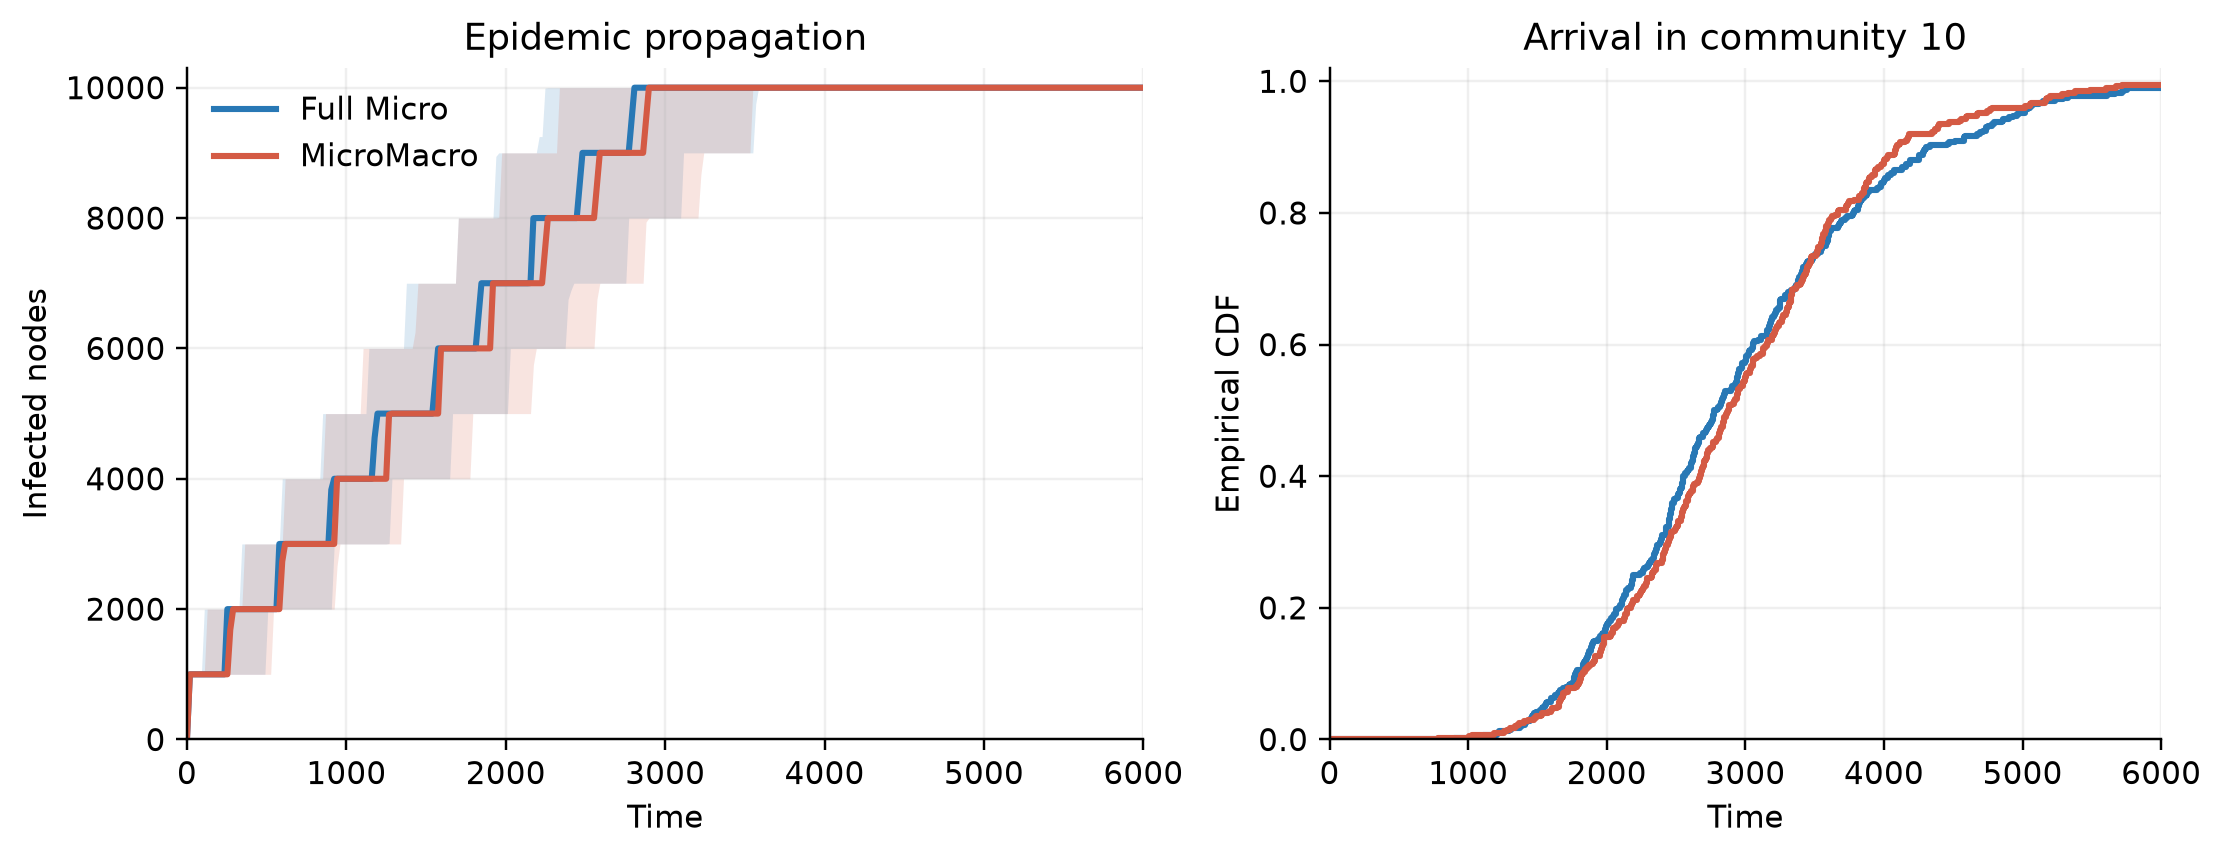
\includegraphics[width=\linewidth]{Images/chain_cliques/chain_cliques_n1000_k1_propagation_cdf_random_initial.png}
\caption{Ланцюг із десяти клік по 1000 вузлів з одним ребром між послідовними кліками ($k=1$, $\beta=0.003$, 400 запусків для кожної моделі). Ліворуч: поточкова медіана кількості інфікованих вузлів із міжквартильними смугами. Праворуч: емпірична функція розподілу часу прибуття до десятої спільноти ($T_9$). Чотири значення прибуття \Full{} і два \TS{} лежать поза показаним діапазоном; усі вони спостережені.}
\label{fig:chain_cliques}
\end{figure}

\subsection{Ланцюги випадкових спільнот}
\label{sec:res_chain_random}

\emph{Розріджені спільноти з довгими шляхами дають систематично ранні прибуття, відносна величина яких залишається сталою вздовж ланцюга, тоді як абсолютне випередження накопичується.} На рисунку~\ref{fig:chain_heatmap} показано кумулятивні часи прибуття у ланцюгах спільнот із 1000 вузлів. Для цільового ASPL 2--3 термінальне $\eW$ становило 1.4--2.5\%, що близько до його вибіркового порога. За ASPL 6 модель \TS{} досягала останньої спільноти раніше на 13.9\% за медіаною для $k=1$ і на 10.7\% для $k=5$ ($\eW=13.6\%$ і 10.9\%). У рядку ASPL 5 за $k=1$ відносне медіанне випередження становило близько 10\% як у першій, так і в останній спільноті, тоді як його абсолютна величина зросла приблизно зі 107 до 1018 одиниць часу. Отже, стала відносна похибка вздовж ланцюга означає зростання абсолютної похибки у віддалених спільнотах. Додатні значення у першому стовпці рядка клік ($+12.6\%$ і $+11.5\%$) не є статистично відмінними від нуля: для $k=1$ зсув середнього першого переходу дорівнює $+4.9\%$ із 95\% інтервалом $[-8.0,18.3]\%$. Для одиничних переходів також характерний вищий вибірковий поріг відстаней, ніж для кумулятивних.

\clearpage
\begin{figure}[H]
\centering
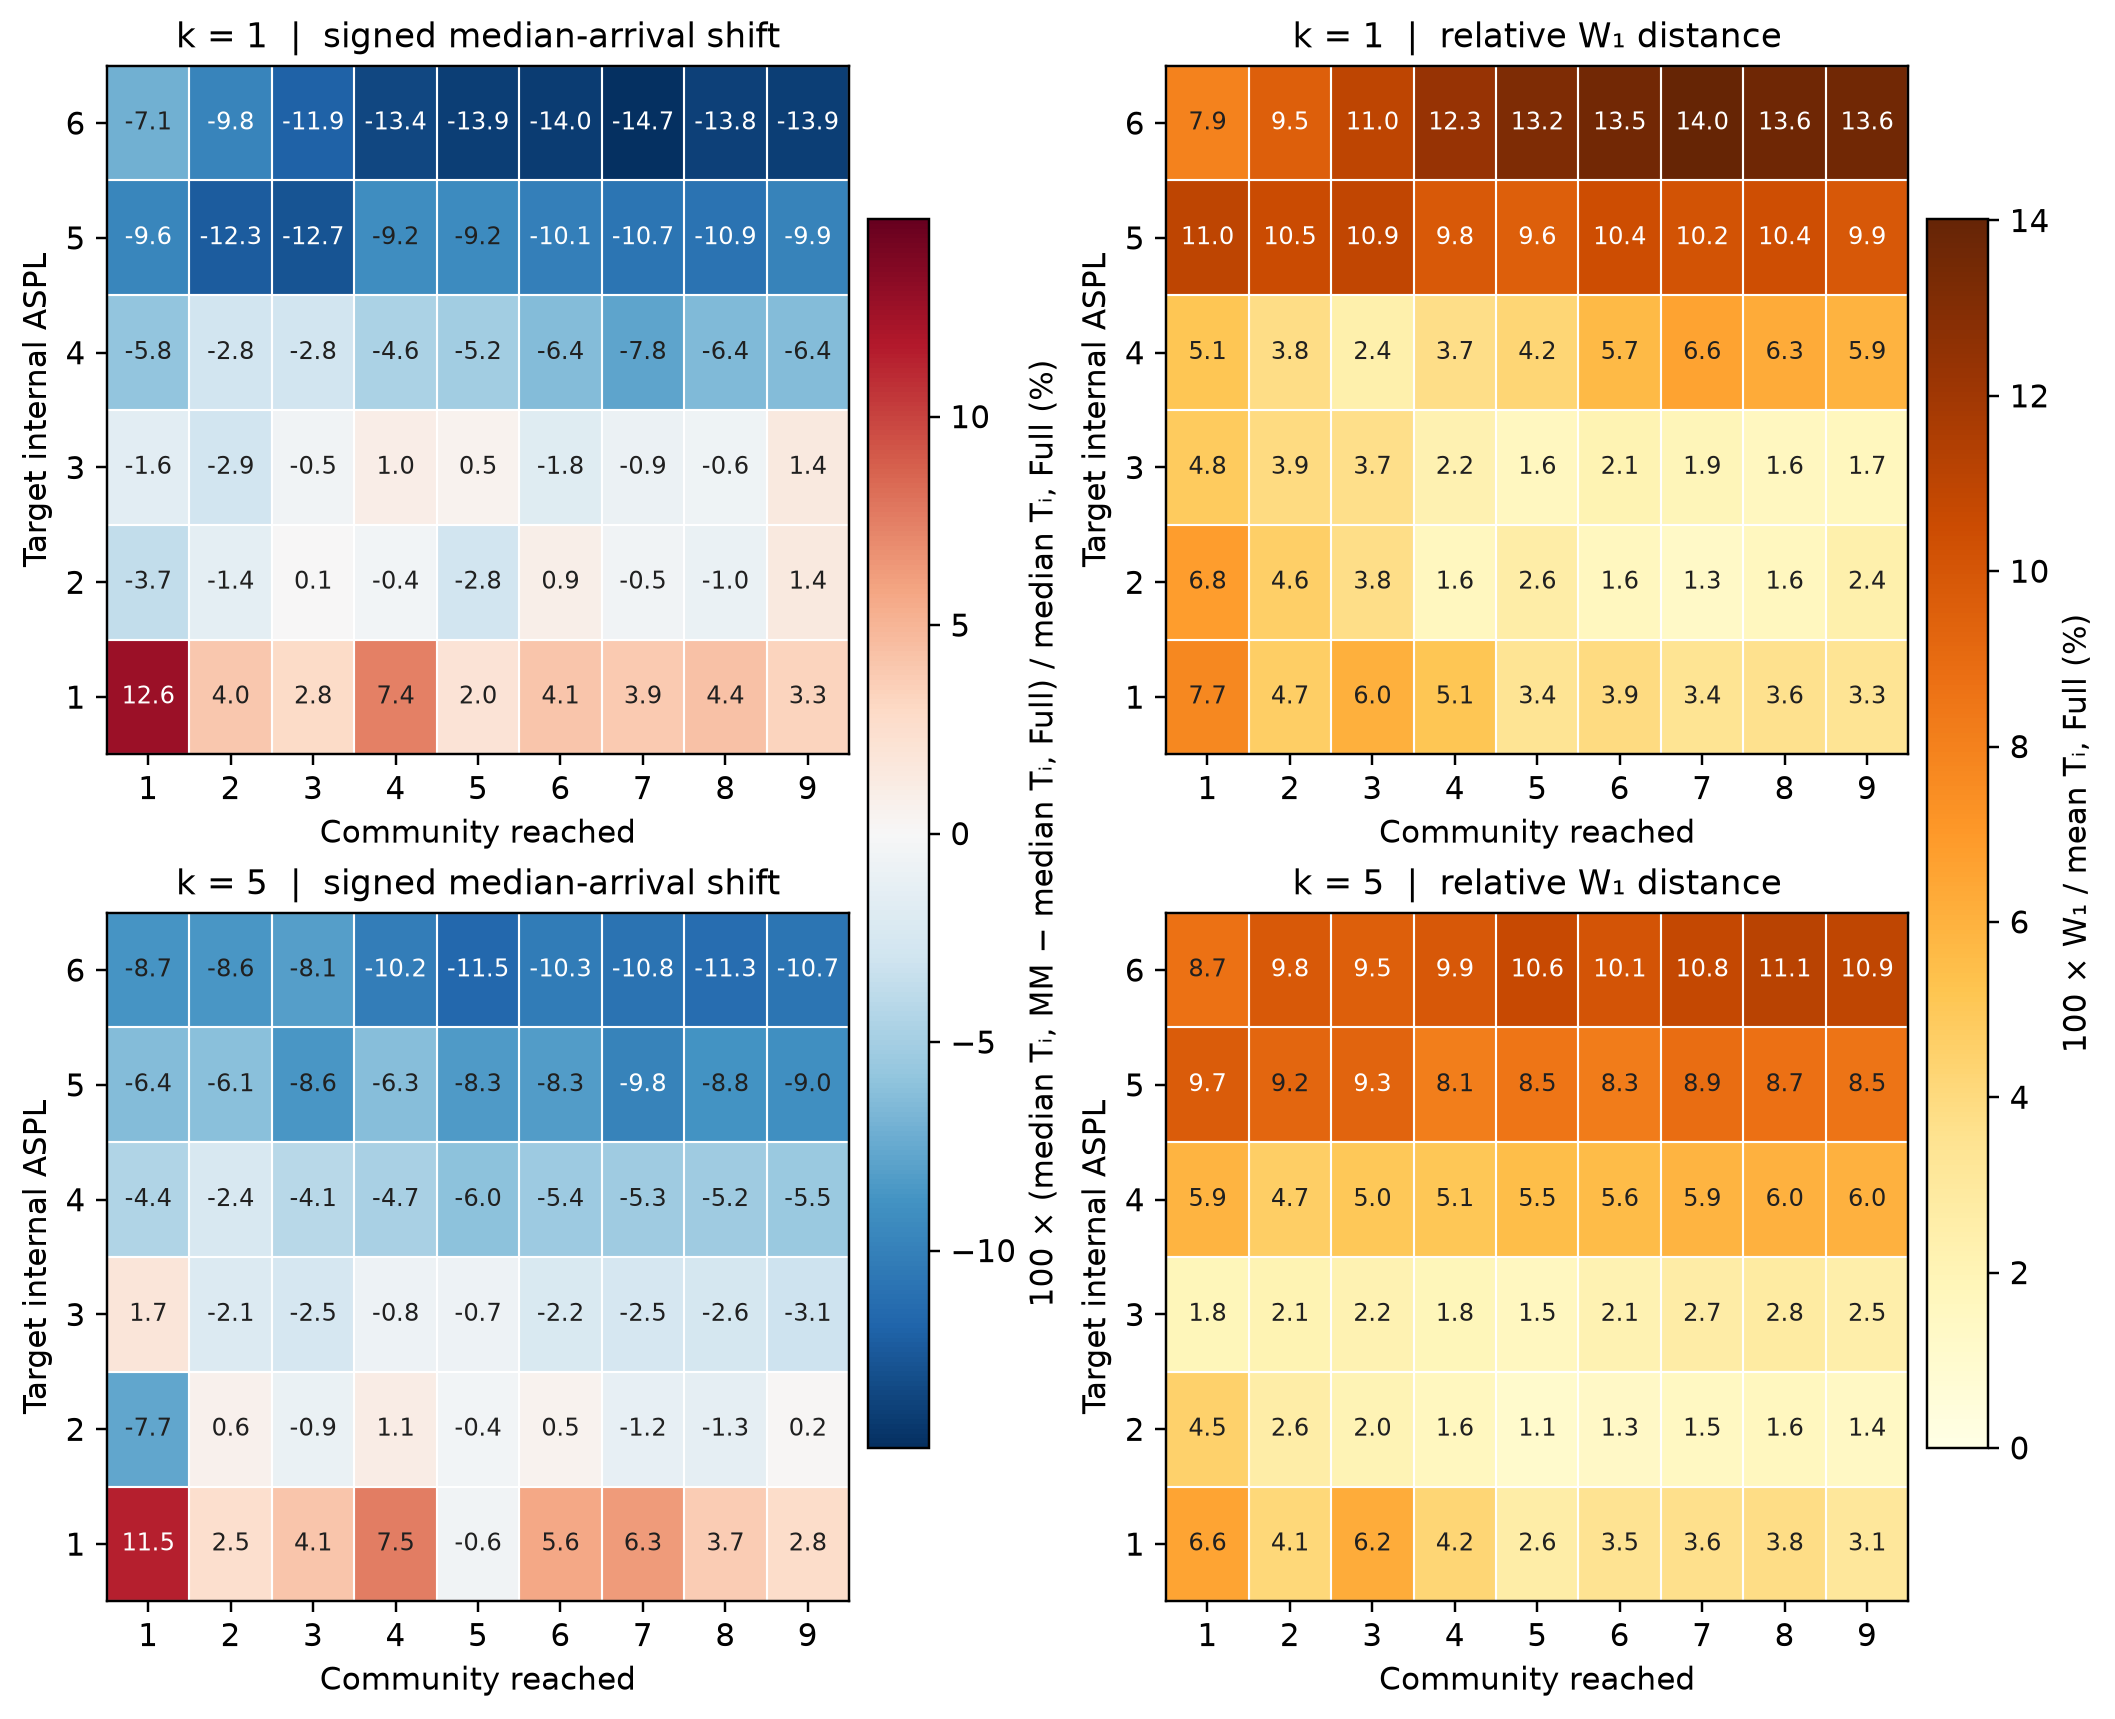
\includegraphics[width=0.82\linewidth]{Images/aspl_chain/aspl_chain_median_arrival_error_map_labeled.png}
\caption{Точність кумулятивних часів прибуття у ланцюгах із десяти спільнот, кожна з яких має $n=1000$ вузлів, залежно від цільового ASPL (рядки) та досягнутої спільноти ($c=1,\dots,9$, стовпці), для $k=1$ (угорі) та $k=5$ (унизу). Ліворуч: відносний зсув медіани $b_c$ (від'ємний: \TS{} прибуває раніше). Праворуч: відносна відстань Васерштайна. Для кожної комірки використано 400 парних запусків; невизначеність не показано (термінальні прибуття див. на рисунку~\ref{fig:accuracy_map}).}
\label{fig:chain_heatmap}
\end{figure}

\subsection{Розмір спільноти та ширина інтерфейсу}
\label{sec:res_size}

\emph{Та сама довжина внутрішнього шляху є значно менш сприятливою в малих спільнотах.} На рисунку~\ref{fig:accuracy_map} наведено термінальну розбіжність для всіх 48 конфігурацій серії за розміром. Пермутаційний поріг був у межах від 1.6\% до 5.9\%. У 16 конфігураціях з ASPL $\le2$ значення $\eW$ становило 1.1--4.4\%, а в 14 із них воно не відрізнялося від порога на рівні значущості 5\%. У 31 із 32 конфігурацій з ASPL $\ge3$ значення $\eW$ перевищувало поріг ($p<0.01$), а зсув медіани був від'ємним із блоковим бутстреп-інтервалом, що не містив нуль. Винятком була конфігурація $n=1000$, ASPL 3, $k=1$, для якої $\eW=1.7\%$. За фіксованого ASPL $\ge3$ розбіжність монотонно зменшувалася зі збільшенням розміру спільноти для обох ширин інтерфейсу. За ASPL 6 значення $\eW$ зменшилося з 41.3\% для $n=50$ до 13.6\% для $n=1000$ за $k=1$, а за $k=5$ --- з 32.4\% до 10.9\%. Ширші інтерфейси зменшували розбіжність у розріджених спільнотах, але не усували її. Частка переходів \TS{}, що передували зараженню будь-якого вузла-моста у спільноті-джерелі, зросла з 0.1--2.3\% за ASPL 1 до 30--52\% за ASPL 6.

\clearpage
\begin{figure}[H]
\centering
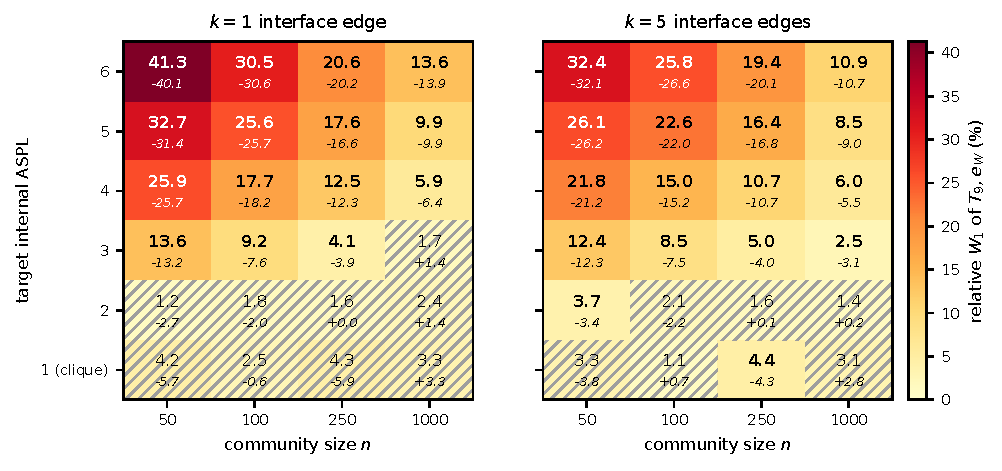
\includegraphics[width=\linewidth]{Images/twoscale/fig_accuracy_map.pdf}
\caption{Точність термінального прибуття у ланцюгах із десяти спільнот для всіх 48 конфігурацій серії за розміром. Колір і напівжирні числа: відносна відстань Васерштайна $\eW$ для $T_9$ (\%). Числа курсивом: відносний зсув медіани $b_9$ (\%; від'ємне значення означає, що \TS{} прибуває раніше). Заштриховані комірки: $\eW$ не відрізняється від внутрішньопарного пермутаційного порога ($p\ge0.05$). Для кожної комірки використано 400 парних запусків.}
\label{fig:accuracy_map}
\end{figure}

\subsection{Єдине співвідношення часових масштабів упорядковує розбіжність}
\label{sec:res_descriptor}

\emph{Якщо виразити результати через $\rho=\beta\sigma_T$, дані для всіх розмірів, структур і ширин інтерфейсу лягають на одну криву.} Для кожної конфігурації ми обчислювали $\sigma_T$ як стандартне відхилення часів зараження вузлів у кожній спільноті-джерелі запусків \Full{}, усереднене за спільнотами й запусками. На рисунку~\ref{fig:descriptor}(a,b) термінальні $\eW$ і $b_9$ зображено залежно від $\rho$. Рангова кореляція між $\eW$ і $\rho$ становила 0.92 для всіх 48 конфігурацій і 0.98 для 32 конфігурацій з ASPL $\ge3$; відповідні значення для цільового ASPL становили 0.82 і 0.67. У 18 конфігураціях із $\rho<0.25$ виконувалося $\eW\le4.4\%$, а 15 із них були нерозрізнюваними з пермутаційним порогом. Усі 30 конфігурацій із $\rho\ge0.25$ були статистично відмінними від порога. Для $\rho\ge0.3$ апроксимація в логарифмічних координатах дала $\eW\approx15\rho\,\%$ (нахил 1.03; медіанне відносне відхилення 8\%, максимальне 41\%) і $b_9\approx-\eW$, тобто розбіжність майже повністю була раннім зсувом. Ми також розглянули два альтернативні масштабування: $\beta\sqrt{k}\sigma_T$, запропоноване виразом~\eqref{eq:hazard_variance}, і середній час від першого зараження спільноти до зараження її першого вузла-моста, помножений на $\beta k$. Обидва розділяли дві ширини інтерфейсу сильніше, ніж $\rho$.

\clearpage
\begin{figure}[H]
\centering
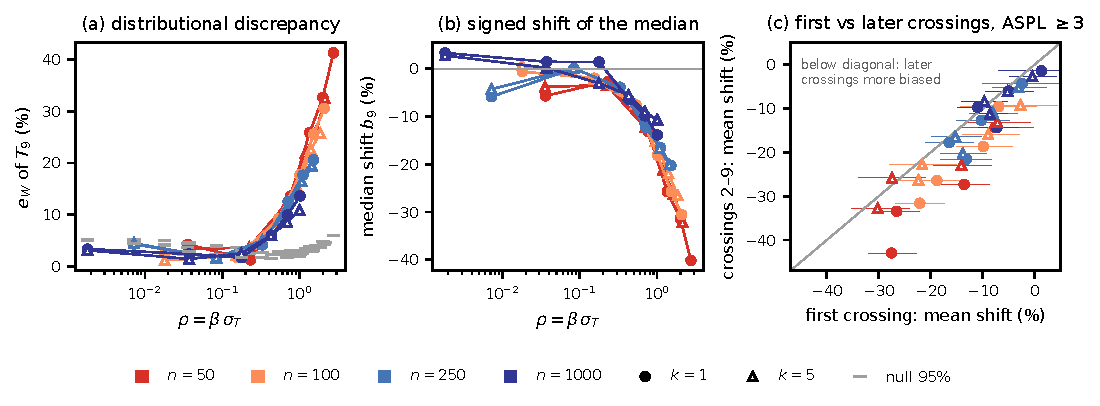
\includegraphics[width=\linewidth]{Images/twoscale/fig_descriptor.pdf}
\caption{(a) Відносна відстань Васерштайна та (b) відносний зсув медіани термінального прибуття залежно від $\rho=\beta\sigma_T$ для всіх 48 конфігурацій ланцюга (кольори: розмір спільноти; зафарбовані кола: $k=1$; порожні трикутники: $k=5$; лінії сполучають ASPL 1--6 за фіксованих $n$ і $k$). Сірі позначки в (a): 95-й процентиль внутрішньопарного пермутаційного порога кожної конфігурації. (c) Локальний середній зсув першого переходу порівняно зі зсувом переходів 2--9 для конфігурацій з ASPL $\ge3$, із 95\% блоковими бутстреп-інтервалами зсуву першого переходу.}
\label{fig:descriptor}
\end{figure}

Рисунок~\ref{fig:descriptor}(c) розділяє окремі переходи. Згідно із зауваженням~\ref{rem:placement}, у нашому дизайні перший перехід залежить лише від механізмів на боці джерела та чисельних механізмів, тоді як наступні переходи також залежать від розміщення після першого імпорту й надлишкових імпортів. Для $k=1$ наступні переходи мали сильніше зміщення, ніж перший, у 15 із 16 конфігурацій з ASPL $\ge3$. Різниця була статистично відмінною від нуля у 9 з них, зокрема для всіх чотирьох розмірів за ASPL 6; наприклад, $-27.5\%$ для першого переходу порівняно з $-42.9\%$ для переходів 2--9 за $n=50$. Для $k=5$ різниця була меншою (14 із 16 точкових оцінок від'ємні, 3 статистично відмінні від нуля). Така залежність від $k$ відповідає передбаченню механізму вичерпання інтерфейсу: одне фізичне ребро допускає один перехід, тоді як п'ять ребер допускають до п'яти, тому надлишкові агреговані імпорти мають менший вплив. Оскільки між конфігураціями використано спільне випадкове засівання, ми вважаємо цю закономірність підтверджувальним, але не остаточним свідченням. Безпосередній підрахунок надлишкових імпортів потребував би журналів типів подій, які не зберігалися.

%======================================================================
\clearpage
\section{Обговорення}
\label{sec:discussion}

\subsection{Практичні рекомендації}

Результати дають змогу запропонувати просту процедуру для визначення того, чи є агреговане зв'язування достатнім.

\paragraph{Визначте, яка спостережувана величина має значення.}
Для часу поширення між спільнотами двомасштабний симулятор може бути точним. Для маршрутів передачі йому довіряти не можна. До половини переходів у розріджених спільнотах і п'ята частина експортів навіть там, де розподіли часу експорту узгоджувалися, відбувалися до зараження будь-якого справжнього вузла-моста. Питання, що залежать від вузлів-мостів, як-от спрямування втручань на осіб, які з'єднують спільноти, або встановлення джерела спалаху, потребують інформації про межу, якої агрегований інтерфейс не містить.

\paragraph{Оцініть співвідношення часових масштабів.}
Обчисліть $\rho=\beta_{\mathrm{out}}\sigma_T$. Оскільки $\sigma_T$ описує поширення в межах однієї спільноти, його в принципі можна оцінити лише за локальними рушіями, моделюючи ізольовану спільноту з рівномірно розміщеним початковим інфікованим вузлом. Ми обчислювали його за еталонними запусками й не перевіряли таку локальну оцінку. У наших тестах термінальні часи прибуття були статистично нерозрізнюваними за $\rho\lesssim0.25$. Для $0.3\lesssim\rho\lesssim3$ модель \TS{} прибувала раніше приблизно на $15\rho\%$. Це правило є емпіричним узагальненням для одного сімейства синтетичних мереж і параметрів, а не загальним законом похибки.

\paragraph{Перевіряйте абсолютні та відносні похибки.}
Уздовж ланцюга відносна розбіжність була майже сталою, тому абсолютне випередження у віддалених спільнотах зростало пропорційно часу поширення. Для визначення часу втручання в конкретній цільовій спільноті релевантною величиною є абсолютна розбіжність у цій спільноті.

\paragraph{Калібруйте відстані відносно вибіркової мінливості.}
За кількох сотень запусків для кожної моделі відстані в кілька відсотків між розподілами часу прибуття очікуються навіть для ідентичних моделей (додаток~\ref{app:floor}). Такі порівняння слід доповнювати пермутаційними базовими рівнями або аналітичними порогами.

\subsection{Обчислювальна вартість}
\label{sec:disc_cost}

Тести було розроблено для оцінювання точності, тому їхні явні інтерфейси містять не більше п'яти ребер, а повна еталонна модель є обчислювально недорогою. У цьому режимі агрегація майже не усуває обчислювальної роботи, а домінує вартість синхронізації на часовій сітці. Медіанний час виконання одного повтору Python-реалізацій був у межах 0.04--0.07\,с (\Full{}) і 0.6--31\,с (\TS{}) для $n=50$ та 8.6--18\,с і 6.7--124\,с відповідно для $n=1000$. Для $n=1000$ відношення двох медіан було в межах від 0.76 (ASPL 2, $k=5$) до 6.9 (ASPL 6, $k=1$). Із цього випливають два висновки. По-перше, коли повна мережа відома й невелика, слід віддавати перевагу \Full{}. По-друге, накладні витрати двомасштабного методу зумовлені планувальником типу «чорна скринька», а не агрегацією. Подієвий планувальник, який точно інтегрує кусково-сталу інтенсивність (розділ~\ref{sec:timing}), усунув би як ці накладні витрати, так і похибку синхронізації. Обчислювальний виграш очікується, коли міжспільнотні контакти численні або недоступні, тобто в умовах, для яких метод і призначено~\citep{kuryliak2025towards}; його кількісне оцінювання залишено для майбутніх досліджень.

\subsection{Обмеження}

В експериментах використано SI-динаміку. За наявності одужання вузли-мости можуть припинити передачу, тоді як частка інфікованих у всій спільноті залишається додатною; у такому разі агрегована інтенсивність також може переоцінювати експорт на пізній стадії локального спалаху. Усі мережі синтетичні, макротопологія є ланцюгом, а внутрішні й зовнішні інтенсивності на ребро однакові. Інтерфейси розміщувалися випадково, що згідно із зауваженням~\ref{rem:placement} нейтралізує похибку розміщення для перших імпортів. Структуровані інтерфейси, наприклад із мостами у вузлах-концентраторах або з віддаленими один від одного вхідними й вихідними мостами, можуть поводитися інакше. Крок синхронізації не варіювали, тому чисельну складову розбіжності не було виокремлено; твердження~\ref{prop:surrogate} дає прямий спосіб зробити це. Нарешті, $\rho$ оцінювали за еталонними запусками й обрали з невеликої кількості можливих масштабувань; його прогностичну цінність для інших сімейств мереж ще потрібно перевірити.

\subsection{Можливі розширення}

Аналіз указує на модифікації, що використовують лише агреговану інформацію. Вичерпання інтерфейсу можна представити, обмеживши кількість імпортів через кожен пучок кількістю його каналів, яка відома, якщо $W_{ij}$ підраховує ребра, або зменшуючи $\lambda_{ij}$ у міру вичерпання цієї місткості. Якщо доступна часткова інформація про межу, $\ibar_i$ у~\eqref{eq:macro_rate} можна замінити часткою інфікованих серед відомих вузлів-мостів. Тоді розміщення можна обмежити відомими кінцевими вузлами-отримувачами. Кожен такий варіант можна порівняти з \Full{} і з точним моделюванням на $\tilde G$, що дає змогу відокремити модельну похибку від чисельної.

%======================================================================
\clearpage
\section{Висновки}
\label{sec:conclusions}

Двомасштабний метод зв'язує точні локальні рушії Gillespie через агреговані інтенсивності між спільнотами. В ідеальній формі він є точним моделюванням на сурогатній мережі, у якій кожен інтерфейс рівномірно розподілено між усіма парами вузлів. Це визначає, яку інформацію метод втрачає: стан справжніх вузлів-мостів, розташування імпортів і скінченну пропускну здатність тонких інтерфейсів. Для випадково розміщених інтерфейсів звідси також випливає, що агреговані годинники експорту стохастично випереджають точні. У контрольованих порівняннях із Gillespie-моделюванням повної мережі розподіли часу термінального прибуття були статистично нерозрізнюваними, коли інфекція поширювалася спільнотами швидко порівняно з часом, потрібним для переходу через ребро інтерфейсу. Коли внутрішній розкид часу наближався до часу такого переходу або перевищував його, двомасштабний симулятор систематично прибував раніше; похибка сягала 40\% у малих розріджених спільнотах. Співвідношення $\rho=\beta\sigma_T$ упорядкувало ці результати для різних розмірів спільнот, внутрішніх структур і ширин інтерфейсу. Близькі часи ніколи не гарантували допустимих маршрутів передачі. Отже, метод є обґрунтованим інструментом для питань про час поширення за малого $\rho$. Він не придатний для питань про індивідуальні маршрути передачі або для розріджених спільнот із довгими внутрішніми шляхами без уточнення інтерфейсу.

%======================================================================
\appendix

\clearpage
\section{Формули для кліки та перевірка}
\label{app:clique}

Розглянемо кліку з $n$ вузлів із SI-динамікою, інтенсивністю $\beta$ на ребро, рівномірно розміщеним початковим інфікованим вузлом і рівномірно вибраною множиною з $k$ вузлів-мостів. Коли заражено $m$ вузлів, наступне внутрішнє зараження відбувається з інтенсивністю $\beta m(n-m)$ незалежно від того, які саме вузли заражені, а множина заражених є рівномірною $m$-підмножиною. Імовірність того, що серед перших $m$ заражених вузлів немає жодного моста, дорівнює $\binom{n-k}{m}/\binom{n}{m}$, отже
\begin{equation}
\label{eq:clique_TB}
\mathbb{E}[T_B]=\sum_{m=1}^{n-k}\frac{\binom{n-k}{m}}{\binom{n}{m}}\frac{1}{\beta m(n-m)},
\qquad
\mathbb{E}[T_B]=\frac{H_{n-1}}{\beta n}\ \ (k=1),
\end{equation}
де $H_{n-1}$ --- гармонічне число; випадок, коли початковий інфікований вузол є мостом ($T_B=0$), також ураховано. Для $k=1$ час експорту у \Full{} дорівнює $T_B$ плюс незалежний час очікування $\Exp(\beta)$. Очікуваний час зараження всієї кліки дорівнює $2H_{n-1}/(\beta n)$. У таблиці~\ref{tab:verification} вираз~\eqref{eq:clique_TB} порівняно з першою спільнотою ланцюгів клік.

\clearpage
\begin{table}[H]
\centering
\caption{Перевірка еталонного симулятора на першій спільноті ланцюгів клік ($\beta=0.003$, 400 запусків для кожної комірки): середній час активації моста та, для $k=1$, середній час очікування після активації (точне значення $1/\beta=333.3$). Наведено середнє $\pm$ стандартна похибка.}
\label{tab:verification}
\small
\begin{tabular}{rrrrr}
\toprule
$n$ & $k$ & $\mathbb{E}[T_B]$, рівн.~\eqref{eq:clique_TB} & середнє $T_B$ у \Full{} & очікування у \Full{} після $T_B$\\
\midrule
50 & 1 & 29.86 & $29.72\pm0.71$ & $354.0\pm16.9$\\
100 & 1 & 17.26 & $17.05\pm0.38$ & $326.5\pm17.0$\\
250 & 1 & 8.13 & $7.84\pm0.15$ & $347.4\pm16.6$\\
1000 & 1 & 2.49 & $2.51\pm0.04$ & $353.8\pm17.9$\\
50 & 5 & 15.97 & $15.96\pm0.55$ & --\\
100 & 5 & 10.31 & $9.64\pm0.29$ & --\\
250 & 5 & 5.35 & $5.16\pm0.12$ & --\\
1000 & 5 & 1.80 & $1.77\pm0.03$ & --\\
\bottomrule
\end{tabular}
\end{table}

\clearpage
\section{Вибірковий поріг відстані Васерштайна}
\label{app:floor}

Нехай $F_R$ і $G_R$ --- емпіричні функції розподілу двох незалежних вибірок розміру $R$ з одного неперервного розподілу $F$. Тоді $W_1=\int|F_R-G_R|\,dx$, а $\sqrt{R}\,(F_R-G_R)$ наближено дорівнює $\sqrt{2}$, помноженому на броунівський міст, обчислений у $F(x)$~\citep{delbarrio1999}. Оскільки $\mathbb{E}|B(u)|=\sqrt{2u(1-u)/\pi}$ для броунівського мосту $B$,
\[
\mathbb{E}[W_1]\approx\frac{2}{\sqrt{\pi R}}\int\sqrt{F(x)\bigl(1-F(x)\bigr)}\,dx .
\]
Для експоненційного розподілу із середнім $\mu$ інтеграл дорівнює $\mu\pi/2$, тому $\mathbb{E}[W_1]/\mu\approx\sqrt{\pi/R}$, що становить 8.9\% для $R=400$ і 1.8\% для $R=10\,000$. Часи прибуття, що є сумами кількох переходів, мають менший розкид відносно свого середнього, а тому й нижчий поріг; пермутаційні пороги конфігурацій ланцюга були в межах від 1.6\% до 5.9\%.

\clearpage
\section{Відомості про відтворюваність}
\label{app:repro}

Значення seed детерміновано отримано з параметрів експерименту. Кожен рушій \TS{} використовує власний потік псевдовипадкових чисел; зондування в середині кроку копіюють стан потоку свого рушія й не просувають його. Два запуски \Full{} ($n=50$, ASPL 6, $k=1$) не досягли десятої спільноти до $T=30\,000$. Їх було повторно запущено до $T=40\,000$ з тими самими графами, початковими вузлами та seed подій. Було перевірено, що їхні історії подій до 30\,000 збігаються зі збереженими запусками, а термінальні прибуття відбулися приблизно в моменти 31\,059 і 31\,007. Значення горизонту не підставляли замість неспостереженої події. Пермутаційний і бутстреп-аналіз конфігурацій ланцюга, дескриптор $\sigma_T$ і рисунки~\ref{fig:accuracy_map}--\ref{fig:descriptor} було обчислено зі збережених запусків скриптами \path{extrascripts/analysis/smpt_twoscale_paper_metrics.py} і \path{extrascripts/visualization/smpt_twoscale_paper_figures.py}.

%======================================================================
\section*{Заява про внесок авторів за CRediT}
\textbf{Yulian Kuryliak:} Концептуалізація, методологія, програмне забезпечення, дослідження, формальний аналіз, візуалізація, написання --- початкова версія. \textbf{Michael T. M. Emmerich:} Концептуалізація, методологія, наукове керівництво, написання --- рецензування та редагування. [Автори мають підтвердити.]

\section*{Декларація про конфлікт інтересів}
Автори заявляють, що їм не відомо про будь-які конкуруючі фінансові інтереси або особисті відносини, які могли б вплинути на роботу, описану в цій статті.

\section*{Фінансування}
[Інформацію про фінансування мають додати автори.]

\section*{Доступність даних}
Код симуляції, збережені результати симуляцій і скрипти аналізу доступні у відповідального автора за обґрунтованим запитом. [Замінити на DOI репозиторію, якщо дані буде депоновано.]

\section*{Декларація про використання генеративного штучного інтелекту та технологій на основі ШІ під час підготовки рукопису}
Під час підготовки цієї роботи автори використовували [назва інструмента або сервісу] з метою [причина]. Після використання цього інструмента або сервісу автори перевірили й за потреби відредагували вміст та беруть на себе повну відповідальність за зміст опублікованої статті. [Автори мають заповнити.]


\bibliographystyle{cas-model2-names}
\bibliography{twoscale_references}
\end{document}
